%!TEX TS-program = xelatex
\documentclass[notes,12pt, aspectratio=169]{beamer}

\usepackage{amsmath,amsfonts,amssymb,amsthm,mathtools}  % пакеты для математики:
%\usepackage{minted}

\usepackage[english, russian]{babel} % выбор языка для документа
\usepackage[utf8]{inputenc} % задание utf8 кодировки исходного tex файла
\usepackage[X2,T2A]{fontenc}        % кодировка

\usepackage{fontspec}         % пакет для подгрузки шрифтов
\setmainfont{Helvetica}  % задаёт основной шрифт документа

% why do we need \newfontfamily:
% http://tex.stackexchange.com/questions/91507/
\newfontfamily{\cyrillicfonttt}{Helvetica}
\newfontfamily{\cyrillicfont}{Helvetica}
\newfontfamily{\cyrillicfontsf}{Helvetica}

\usepackage{unicode-math}     % пакет для установки математического шрифта
% \setmathfont{Neo Euler} % шрифт для математики

\usepackage{polyglossia}      % Пакет, который позволяет подгружать русские буквы
\setdefaultlanguage{russian}  % Основной язык документа
\setotherlanguage{english}    % Второстепенный язык документа

% Шрифт для кода
\setmonofont[Scale=0.85]{Monaco}
\usepackage{verbments}

\usepackage{pgfpages}
% These slides also contain speaker notes. You can print just the slides,
% just the notes, or both, depending on the setting below. Comment out the want
% you want.
%\setbeameroption{hide notes} % Only slide
%\setbeameroption{show only notes} % Only notes
%\setbeameroption{show notes on second screen=right} % Both

\usepackage{array}

\usepackage{tikz}
\usepackage{verbatim}
\setbeamertemplate{note page}{\pagecolor{yellow!5}\insertnote}
\usetikzlibrary{positioning}
\usetikzlibrary{snakes}
\usetikzlibrary{calc}
\usetikzlibrary{arrows}
\usetikzlibrary{decorations.markings}
\usetikzlibrary{shapes.misc}
\usetikzlibrary{matrix,shapes,arrows,fit,tikzmark}

\usepackage{hyperref}
\usepackage{lipsum}
\usepackage{multimedia}
\usepackage{multirow}
\usepackage{dcolumn}
\usepackage{bbm}
\newcolumntype{d}[0]{D{.}{.}{5}}

\usepackage{changepage}
\usepackage{appendixnumberbeamer}
\newcommand{\beginbackup}{
   \newcounter{framenumbervorappendix}
   \setcounter{framenumbervorappendix}{\value{framenumber}}
   \setbeamertemplate{footline}
   {
     \leavevmode%
     \hline
     box{%
       \begin{beamercolorbox}[wd=\paperwidth,ht=2.25ex,dp=1ex,right]{footlinecolor}%
%         \insertframenumber  \hspace*{2ex} 
       \end{beamercolorbox}}%
     \vskip0pt%
   }
 }
\newcommand{\backupend}{
   \addtocounter{framenumbervorappendix}{-\value{framenumber}}
   \addtocounter{framenumber}{\value{framenumbervorappendix}} 
}

% для имитации питоновского синтаксиса 
\newcommand{\pgr}[1]{{\color{green} \textbf{#1}}}


%%%%%%%%%% Работа с картинками %%%%%%%%%
\usepackage{graphicx}                  % Для вставки рисунков
\usepackage{graphics}
\graphicspath{{images/}}    % можно указать папки с картинками
\usepackage{wrapfig}                   % Обтекание рисунков и таблиц текстом

\usepackage[space]{grffile}
\usepackage{booktabs}

% These are my colors -- there are many like them, but these ones are mine.
\definecolor{blue}{RGB}{0,114,178}
\definecolor{red}{RGB}{213,94,0}
\definecolor{yellow}{RGB}{240,228,66}
\definecolor{green}{RGB}{0,128, 0}

\hypersetup{
  colorlinks=false,
  linkbordercolor = {white},
  linkcolor = {blue}
}


%% I use a beige off white for my background
\definecolor{MyBackground}{RGB}{255,253,218}

%% Uncomment this if you want to change the background color to something else
%\setbeamercolor{background canvas}{bg=MyBackground}

%% Change the bg color to adjust your transition slide background color!
\newenvironment{transitionframe}{
  \setbeamercolor{background canvas}{bg=yellow}
  \begin{frame}}{
    \end{frame}
}

\setbeamercolor{frametitle}{fg=blue}
\setbeamercolor{title}{fg=black}
\setbeamertemplate{footline}[frame number]
\setbeamertemplate{navigation symbols}{} 
\setbeamertemplate{itemize items}{-}
\setbeamercolor{itemize item}{fg=blue}
\setbeamercolor{itemize subitem}{fg=blue}
\setbeamercolor{enumerate item}{fg=blue}
\setbeamercolor{enumerate subitem}{fg=blue}
\setbeamercolor{button}{bg=MyBackground,fg=blue,}


% If you like road maps, rather than having clutter at the top, have a roadmap show up at the end of each section 
% (and after your introduction)
% Uncomment this is if you want the roadmap!
% \AtBeginSection[]
% {
%    \begin{frame}
%        \frametitle{Roadmap of Talk}
%        \tableofcontents[currentsection]
%    \end{frame}
% }
\setbeamercolor{section in toc}{fg=blue}
\setbeamercolor{subsection in toc}{fg=red}
\setbeamersize{text margin left=1em,text margin right=1em} 

% списки, которые растягиваются на всю величину слайда 
\newenvironment{wideitemize}{\itemize\addtolength{\itemsep}{10pt}}{\enditemize}

\DeclareMathOperator{\Var}{Var}
\DeclareMathOperator{\E}{E}

\title[]{\textcolor{blue}{Глубокое обучение и вообще}}
\author{Ульянкин Филипп}
\date{\today}

\usepackage{ulem}

\begin{document}

%%% TIKZ STUFF
\tikzset{   
        every picture/.style={remember picture,baseline},
        every node/.style={anchor=base,align=center,outer sep=1.5pt},
        every path/.style={thick},
        }
\newcommand\marktopleft[1]{%
    \tikz[overlay,remember picture] 
        \node (marker-#1-a) at (-.3em,.3em) {};%
}
\newcommand\markbottomright[2]{%
    \tikz[overlay,remember picture] 
        \node (marker-#1-b) at (0em,0em) {};%
}
\tikzstyle{every picture}+=[remember picture] 
\tikzstyle{mybox} =[draw=black, very thick, rectangle, inner sep=10pt, inner ysep=20pt]
\tikzstyle{fancytitle} =[draw=black,fill=red, text=white]
%%%% END TIKZ STUFF

% Title Slide


\begin{frame}
\maketitle
\centering \textbf{\color{blue} Посиделка 7:}  оптимизация и эвристики
\end{frame}

\begin{frame}{В предыдущих сериях: активация} 
\begin{center}
	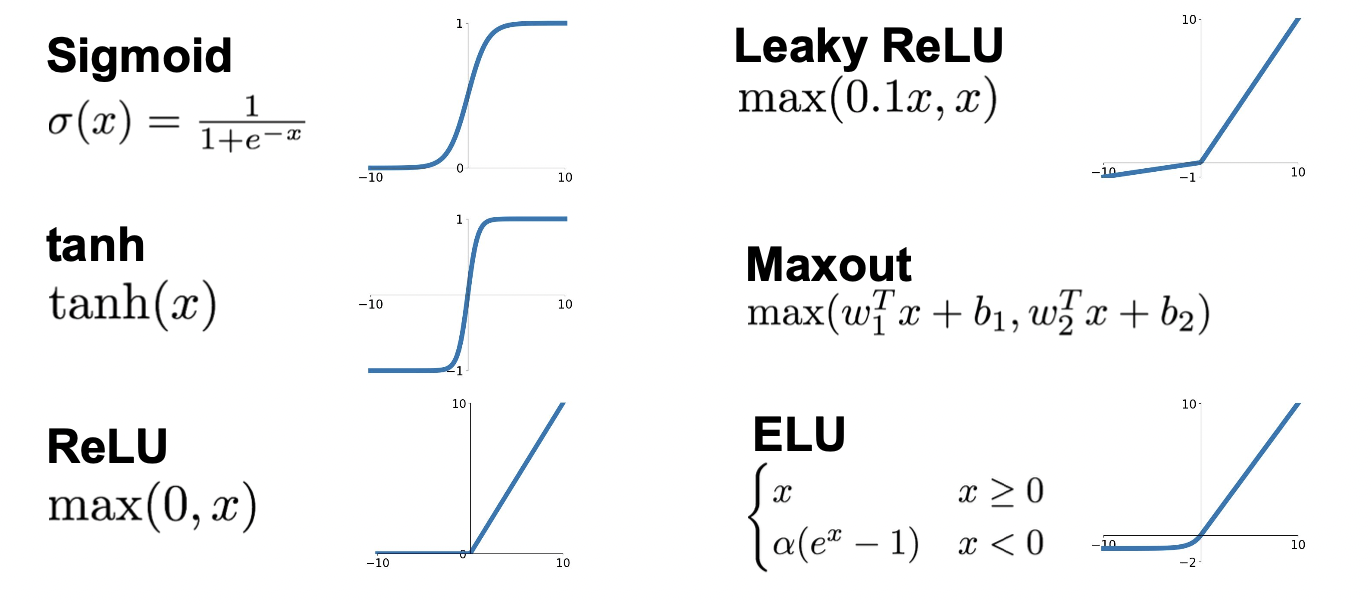
\includegraphics[width=.95\linewidth]{prev_activation.png}
\end{center}
\end{frame}


\begin{frame}{В предыдущих сериях: инициализация} 
\begin{center}
	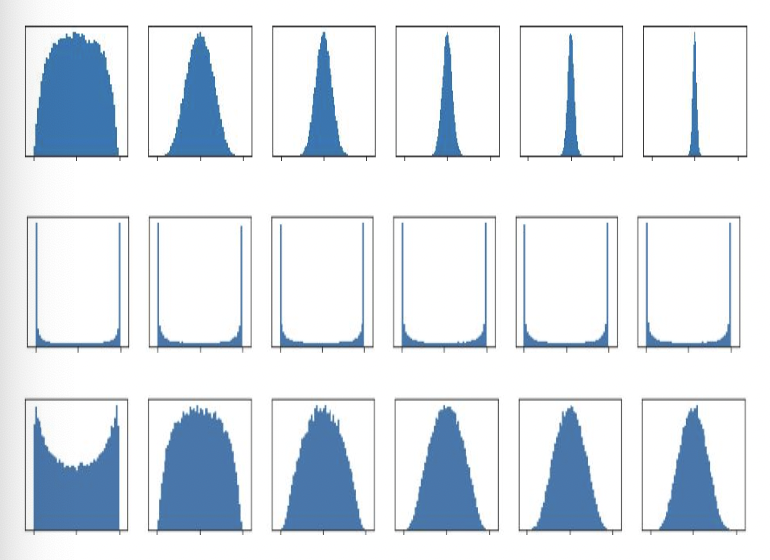
\includegraphics[width=.7\linewidth]{prev_init.png}
\end{center}
\end{frame}


\begin{frame}{В предыдущих сериях: предобработка} 
\begin{center}
	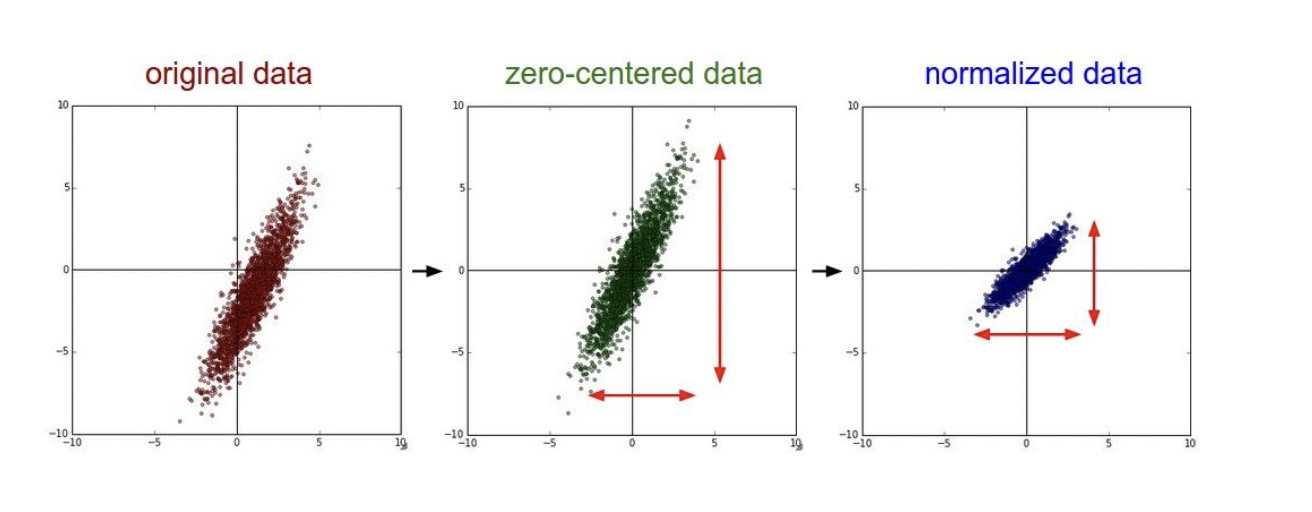
\includegraphics[width=.9\linewidth]{prev_prep.png}
\end{center}
\end{frame}

\begin{frame}{В предыдущих сериях: регуляризация} 
\begin{center}
	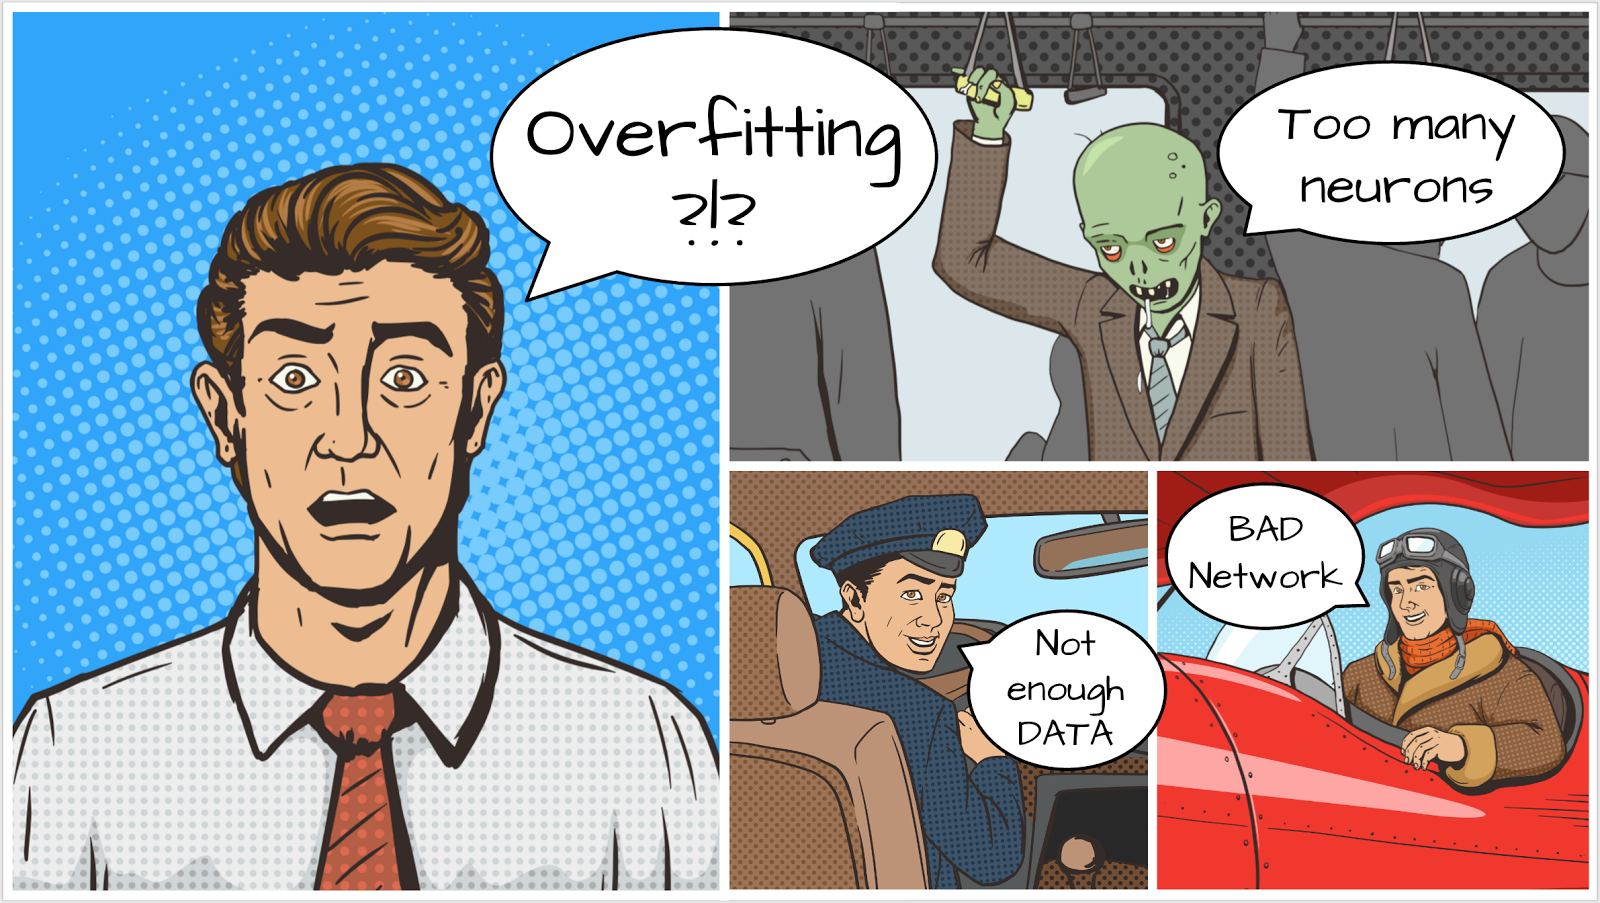
\includegraphics[width=.9\linewidth]{prev_overfitting.png}
\end{center}
\end{frame}

\begin{frame}{В предыдущих сериях: 50 оттенков градиентного спуска} 
\begin{center}
	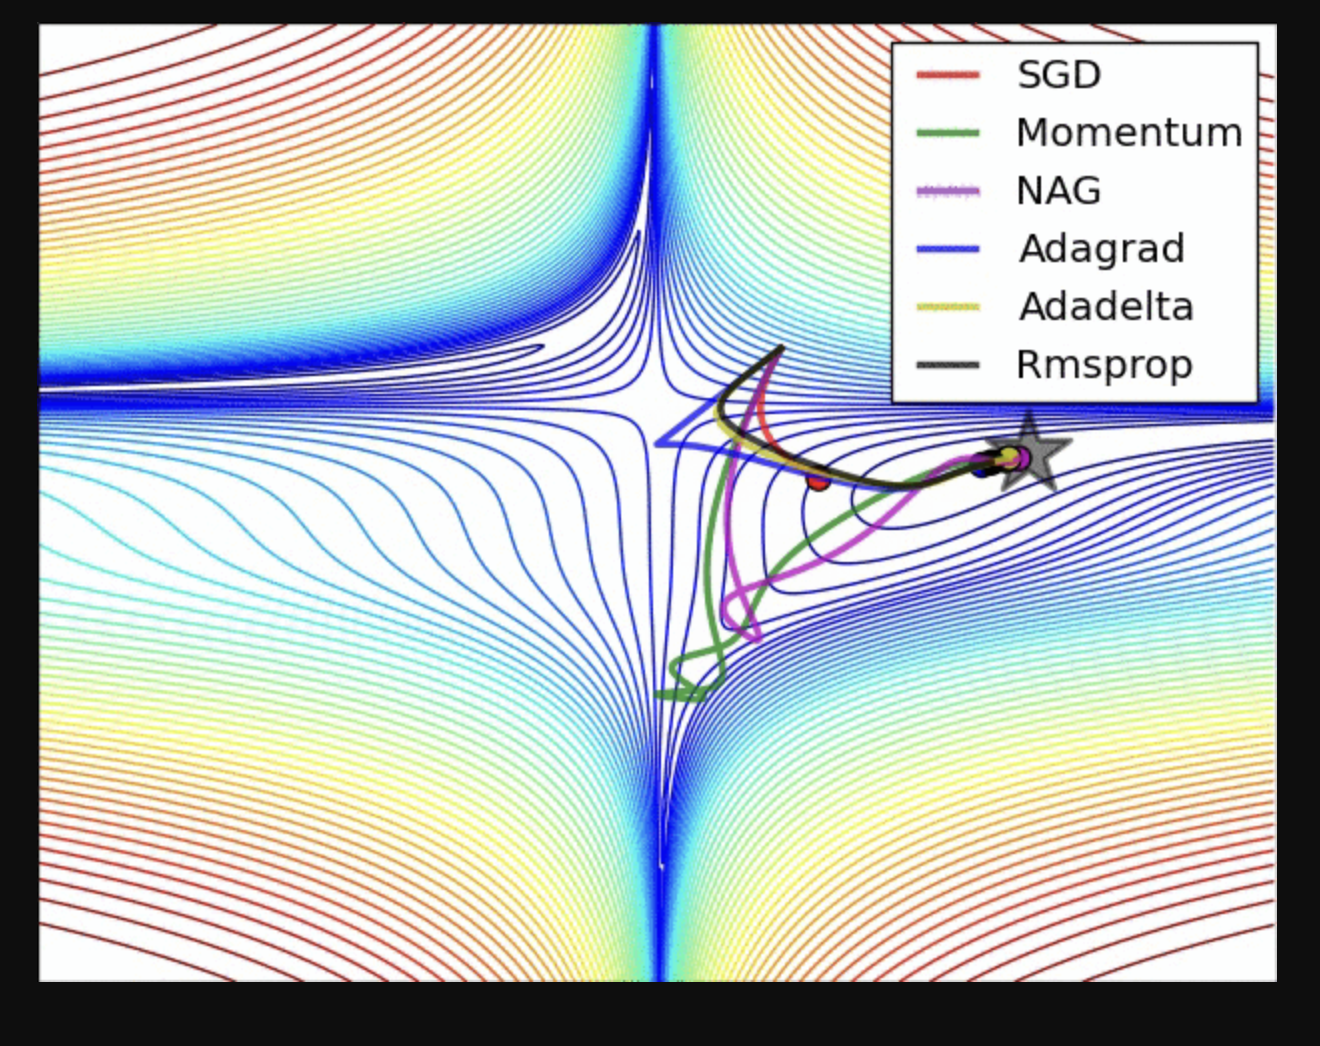
\includegraphics[width=.55\linewidth]{prev_grad.png}
\end{center}
\end{frame}


\begin{frame}{Agenda}
\begin{wideitemize}
%	\item Градиентный спуск: на 50 оттенков темнее
	\item Ландшафт функции потерь 
	\item Нормализация по батчам 
%	\item чёт ещё лол (Стэнфорд)
	\item Организация DL-экспериментов 
\end{wideitemize}
\end{frame}



\begin{transitionframe}
	\begin{center}
		\Huge Ландшафт функции потерь
	\end{center}
%	\centering 
\includegraphics[scale = 0.1]{shadows50.jpg}
\end{transitionframe}


\begin{frame}{Боб чилит в локальном минимуме}
	\begin{center}
		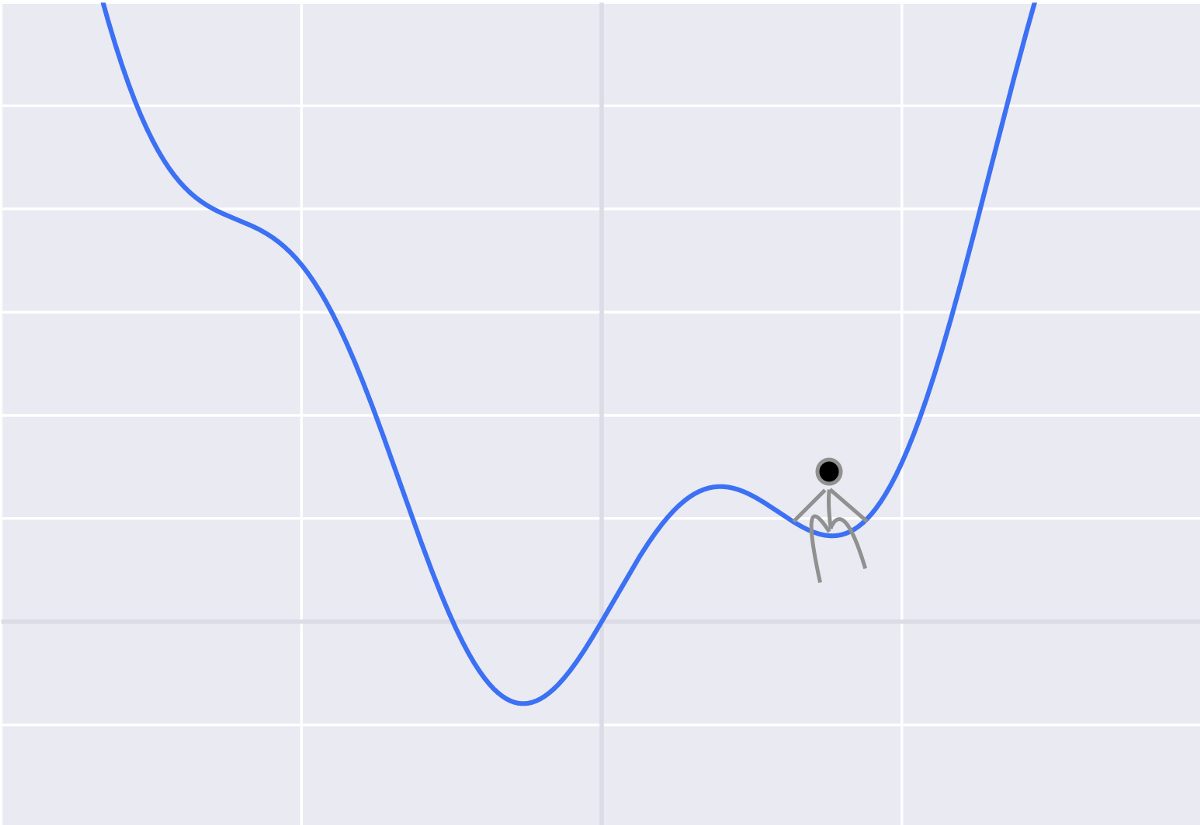
\includegraphics[width=0.6\paperwidth]{bob_local_chill.png}
	\end{center}
	\vfill %
	\footnotesize 
	\color{blue} \url{https://hackernoon.com/life-is-gradient-descent-880c60ac1be8}
\end{frame}


\begin{frame}{Седловые точки}
	\begin{center}
		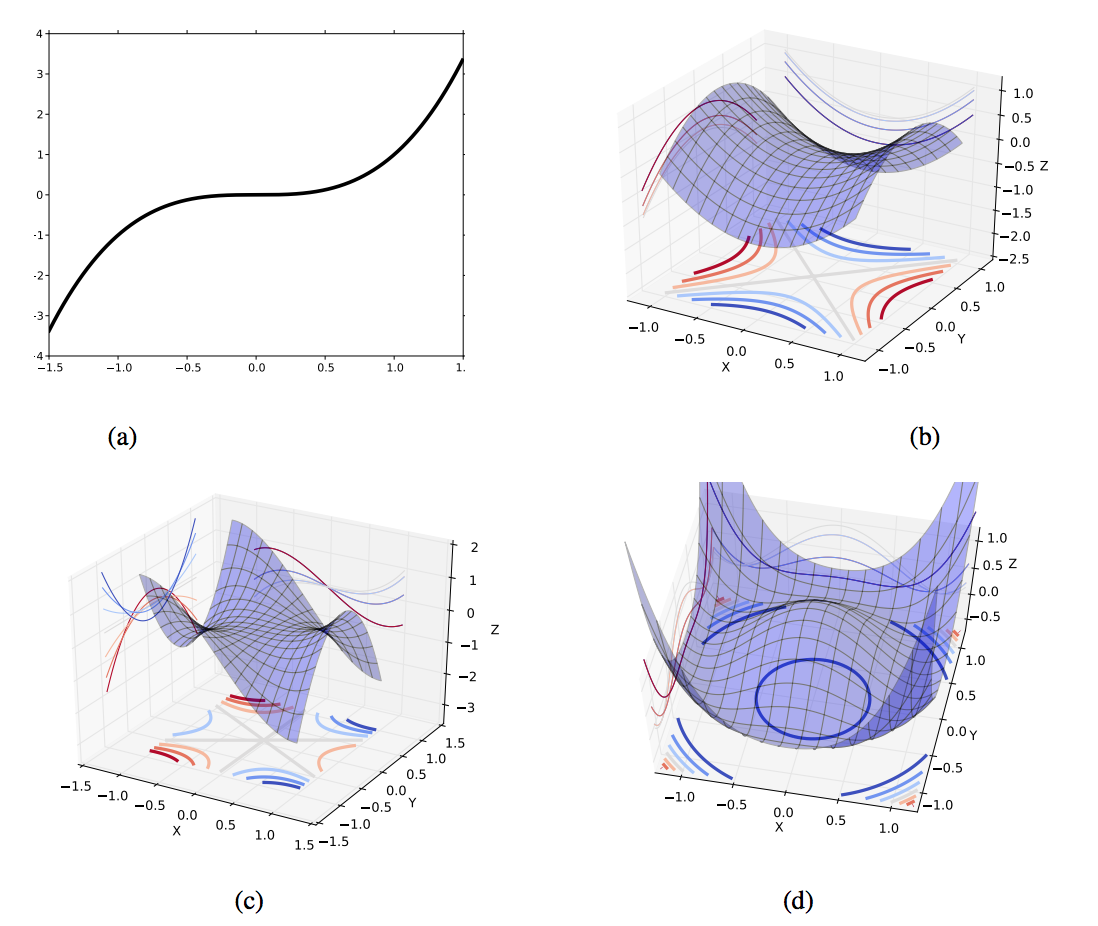
\includegraphics[width=0.5\paperwidth]{sedlo.png}
	\end{center}
	\vfill %
	\footnotesize 
	\color{blue} \url{https://arxiv.org/pdf/1406.2572.pdf}
\end{frame}


\begin{frame}{Визуализация потерь}
	\begin{center}
		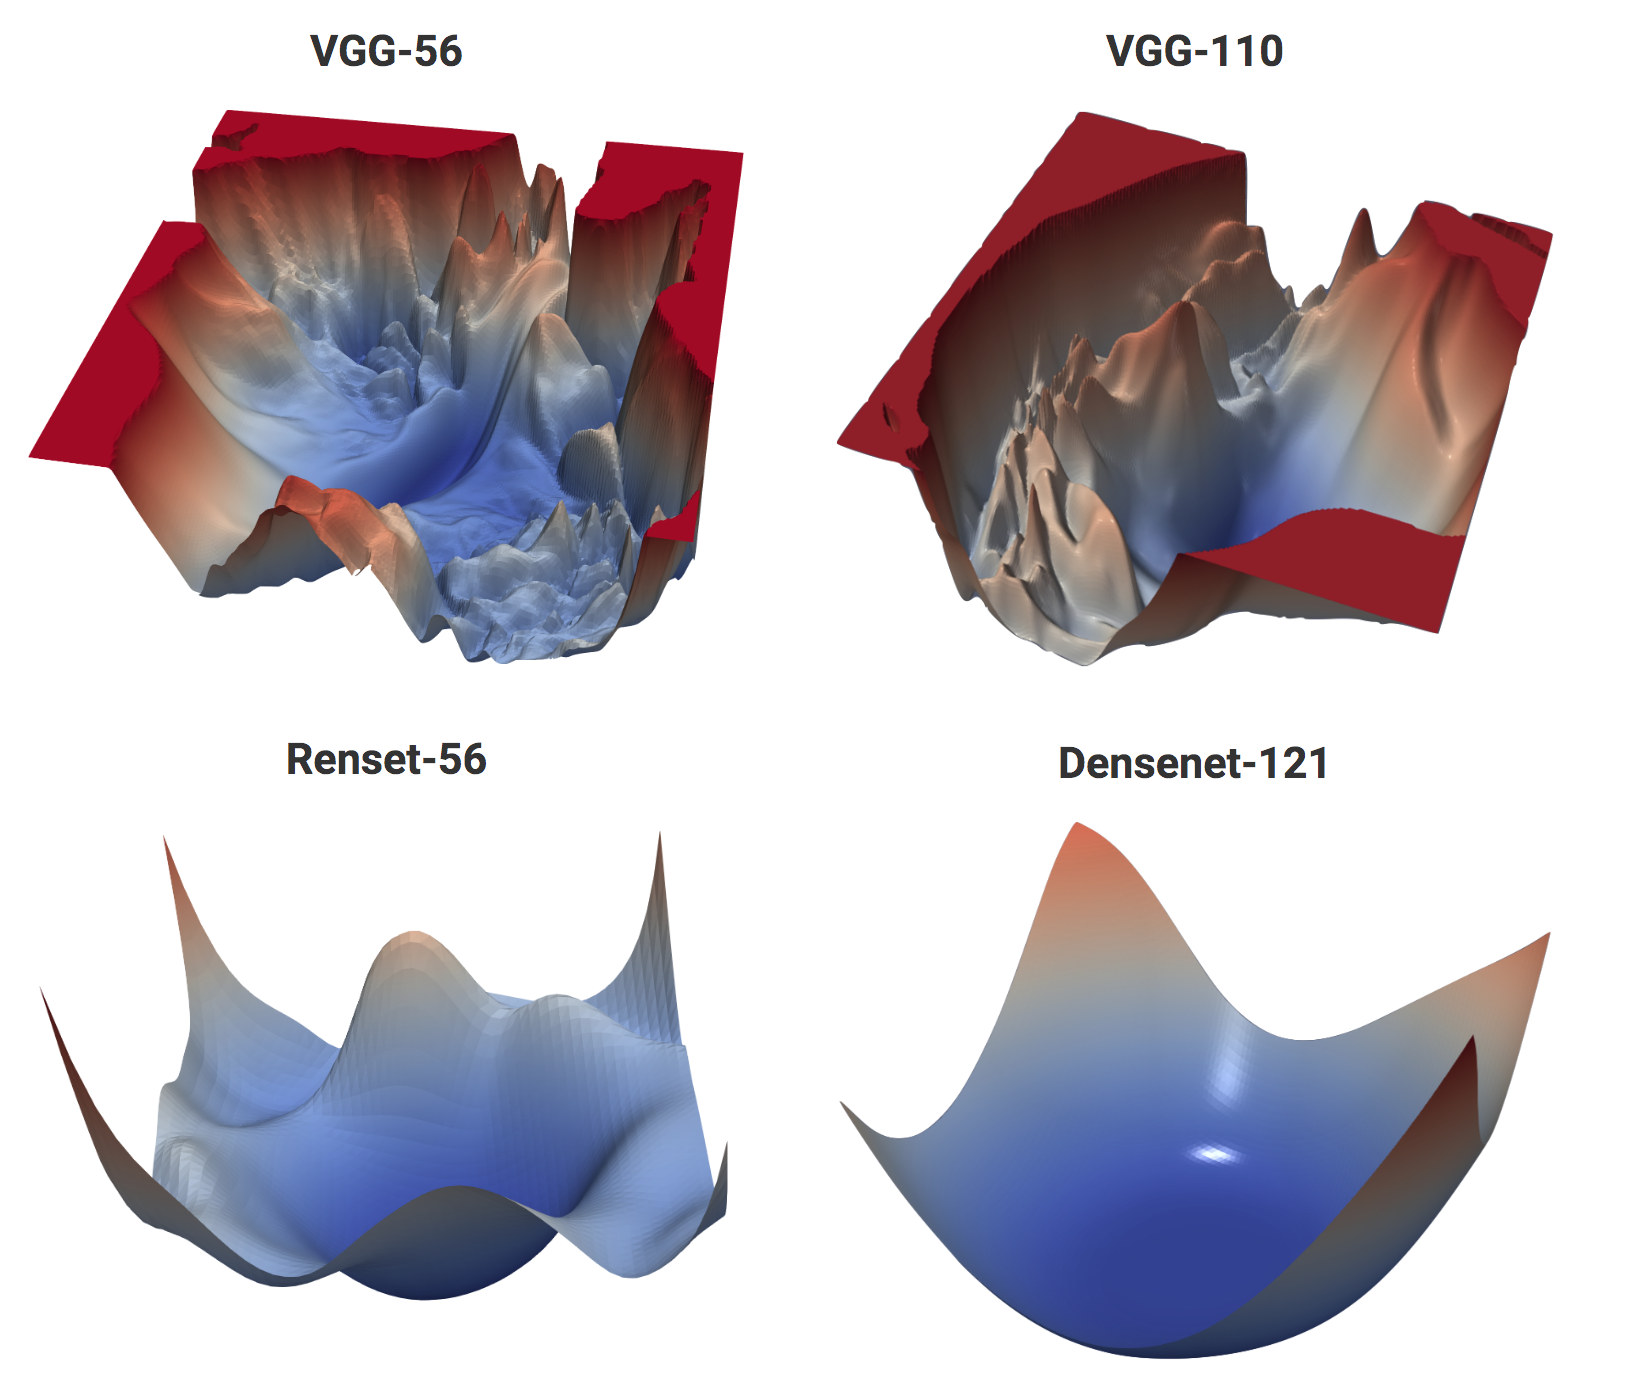
\includegraphics[width=0.5\paperwidth]{loss.png}
	\end{center}
	\vfill %
	\footnotesize 
	\color{blue} \url{https://arxiv.org/pdf/1712.09913.pdf} \newline  \url{https://github.com/tomgoldstein/loss-landscape}
\end{frame}


\begin{frame}{Визуализация потерь}
 Подробнее про это!
 
 Обновить слайды про циклическую скорость, если честно это хуйня полная, добавить нормальные слайды про параболы да берты 
\end{frame}


\begin{frame}{Циклическая скорость обучения (CLR)}
	\begin{wideitemize}
		\item Хочется, чтобы был шанс вылезти из локального минимума, а также шанс сползти с седла $\Rightarrow$ давайте менять глобальную скорость обучения циклически
	\end{wideitemize}
	\begin{center}
		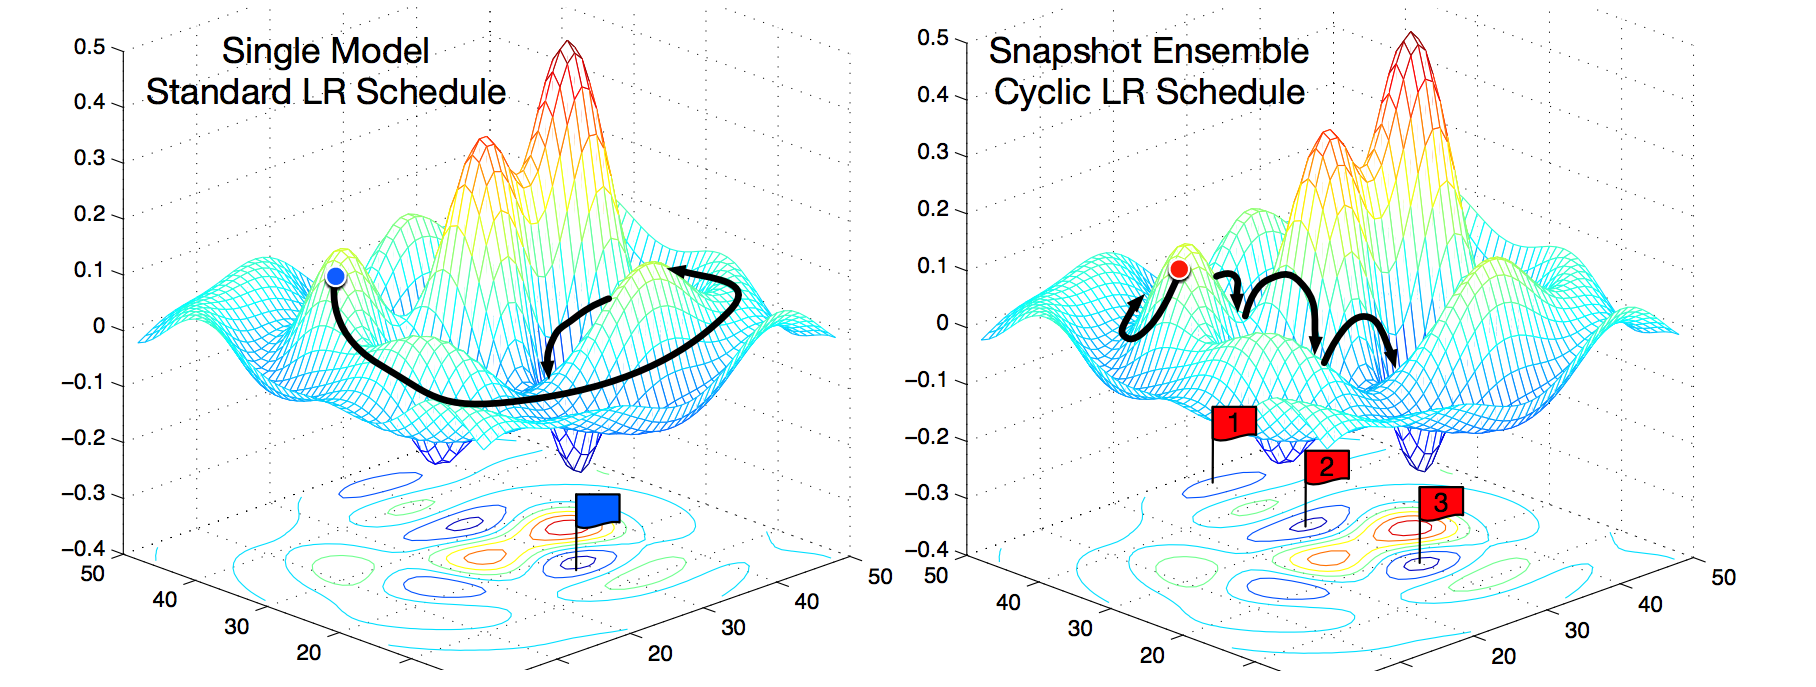
\includegraphics[width=0.7\paperwidth]{cycle_sgd.png}
	\end{center}
\end{frame}


\begin{frame}{Циклическая скорость обучения (CLR)}
	\begin{columns}[T] % align columns
	\begin{column}{.48\textwidth}
		\centering 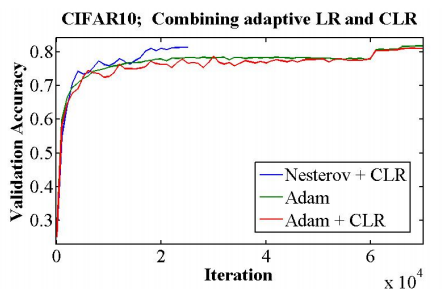
\includegraphics[scale=0.55]{cycle_2.png}
	\end{column}%
	\hfill%
	\begin{column}{.48\textwidth}
	\centering 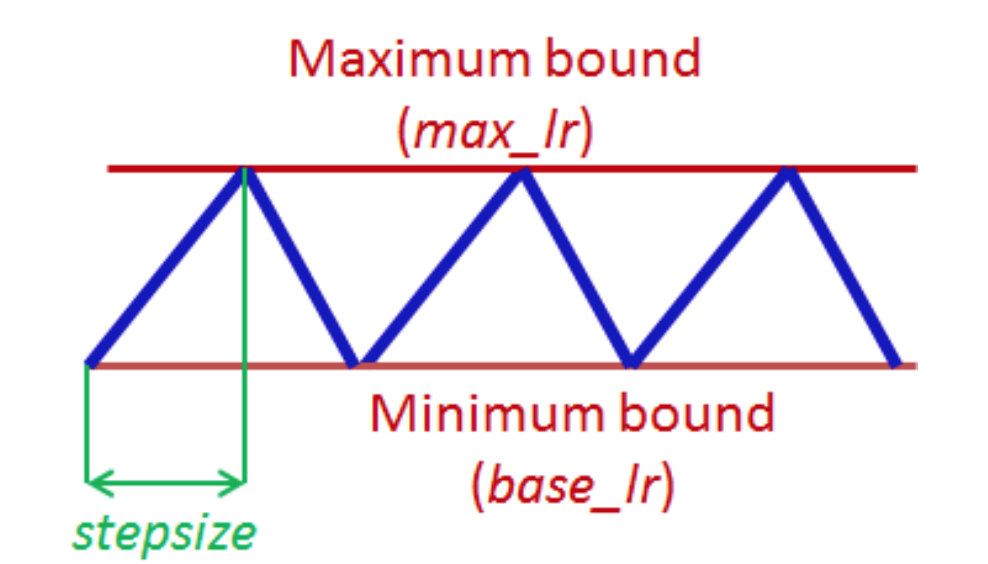
\includegraphics[scale=0.17]{cycle.png} \\ \mbox{ } \\
	Нестеров с CLR отработал \\ быстрее и лучше Adam \\ \alert{Нет одного правильного \\ алгоритма на все случаи!}  \\ Всегда надо экспериментировать
	\end{column}%
	\end{columns}
	
	\vfill %
	\footnotesize  
	\color{blue} \url{https://arxiv.org/pdf/1506.01186.pdf} \newline  \url{https://openreview.net/pdf?id=BJYwwY9ll}
\end{frame}


\begin{frame}{LR range test aka LRFinder}
	\begin{wideitemize}
		\item   Эвристика для подбора learning rate 
		
		\item  Увеличиваем learning rate после каждого батча, остановка перед взрывом значений loss-функции
		
		\item  Есть готовые реализации (в том числе в pytorch и tensorflow) 
		
		\item  Аналогично можно искать оптимальное значение для momentum
	\end{wideitemize}
	\vfill
	
	\footnotesize
	{\color{blue} \url{https://sgugger.github.io/how-do-you-find-a-good-learning-rate.html} \newline 
		\url{https://arxiv.org/abs/1506.01186} \newline 
		\url{https://arxiv.org/abs/1803.09820}}
\end{frame}


% ToDO: 
% Сюда про скорости обучения и их изменение из стэнфорда 
% Слайд про обучение модели со всеми фиксированными весами кроме батчнорма



\begin{transitionframe}
	\begin{center}
		\Huge  Батч-нормализация
	\end{center}
	\centering 
\includegraphics[scale = 0.25]{batcAlice.png}
\end{transitionframe}


\begin{frame}{Стандартизация}
	\begin{center}
		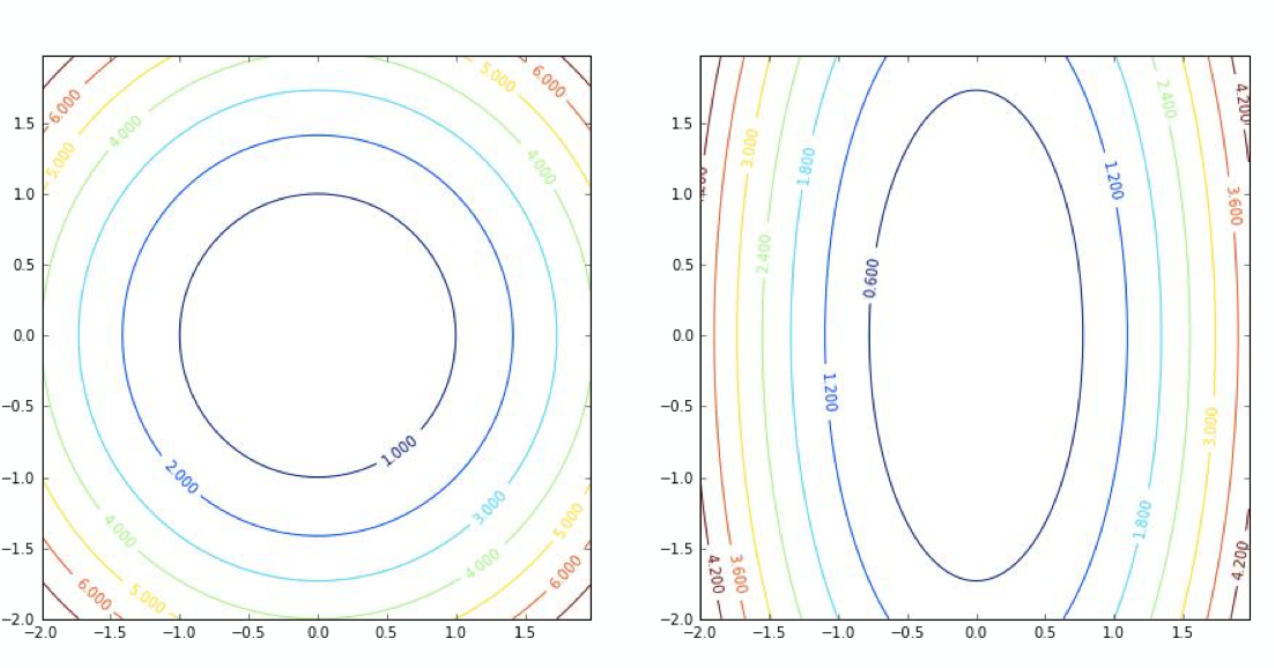
\includegraphics[width=.8\linewidth]{standartization.png}
	\end{center}
	
	\begin{center}
		Какая из ситуаций лучше для градиентного спуска? 
	\end{center}
\end{frame}


\begin{frame}{Стандартизация}
	\begin{center}
		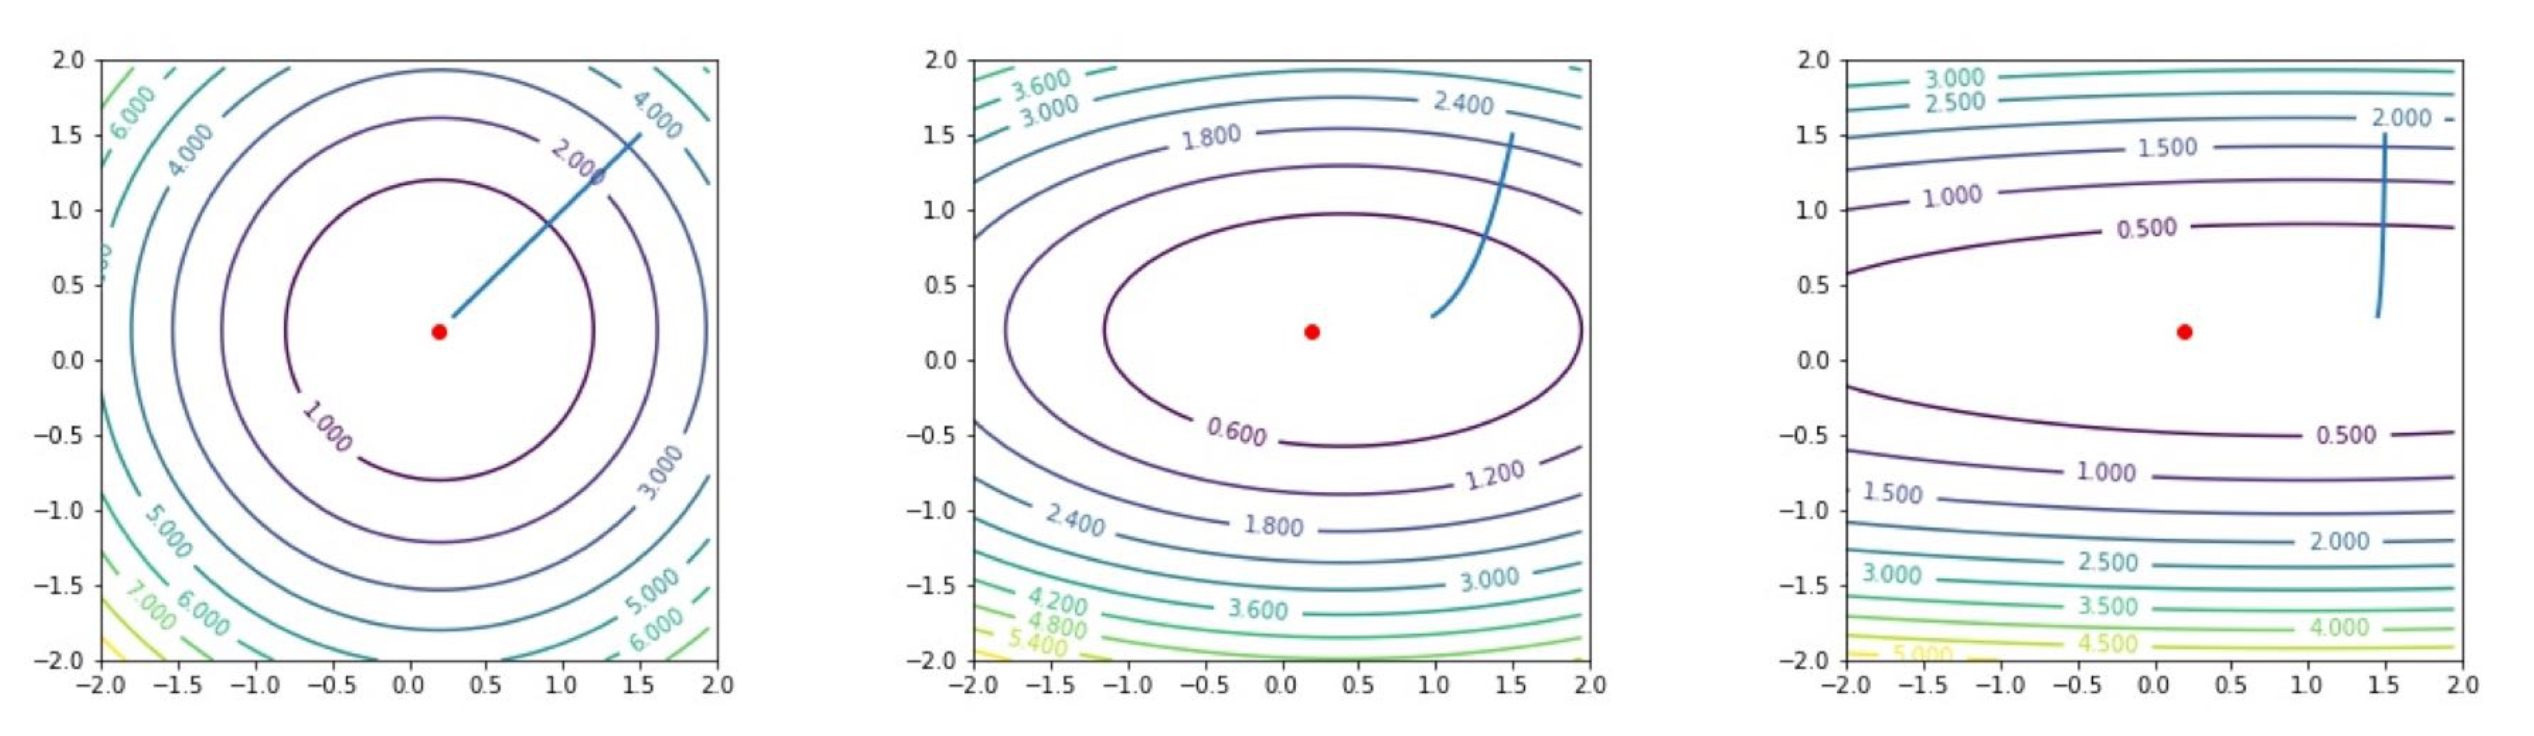
\includegraphics[width=.99\linewidth]{standartization2.png}
	\end{center}
	
	\alert{Градиентные методы быстрее сходятся, если градиенты в одном масштабе}
	
	\vfill %
	\footnotesize
	{\color{blue} \url{https://github.com/hse-aml/intro-to-dl/blob/master/week2/v2/ill-conditioned-demo.ipynb}}
\end{frame}


\begin{frame}{Стандартизация}
Будем подавать на вход в нейросетку стандартизованные данные:

\begin{equation*}
	\begin{aligned}
		&x_{ij}^{*} = \frac{x_{ij} - \hat{\mu}_j}{\sqrt{\hat{\sigma}^2_j + \varepsilon}} \\
		&\hat{\mu_j} = \frac{1}{n} \sum_{i=1}^n x_{ij} \\
		& \hat{\sigma}^2_j =  \frac{1}{n} \sum_{i=1}^n (x_{ij} - \hat{\mu}_j)^2
	\end{aligned}
\end{equation*}
\vfill \centering
\alert{Это помогает градиентному спуску лучше работать}
\end{frame}


\begin{frame}{А что внутри нейросетки?}
	\begin{center}
		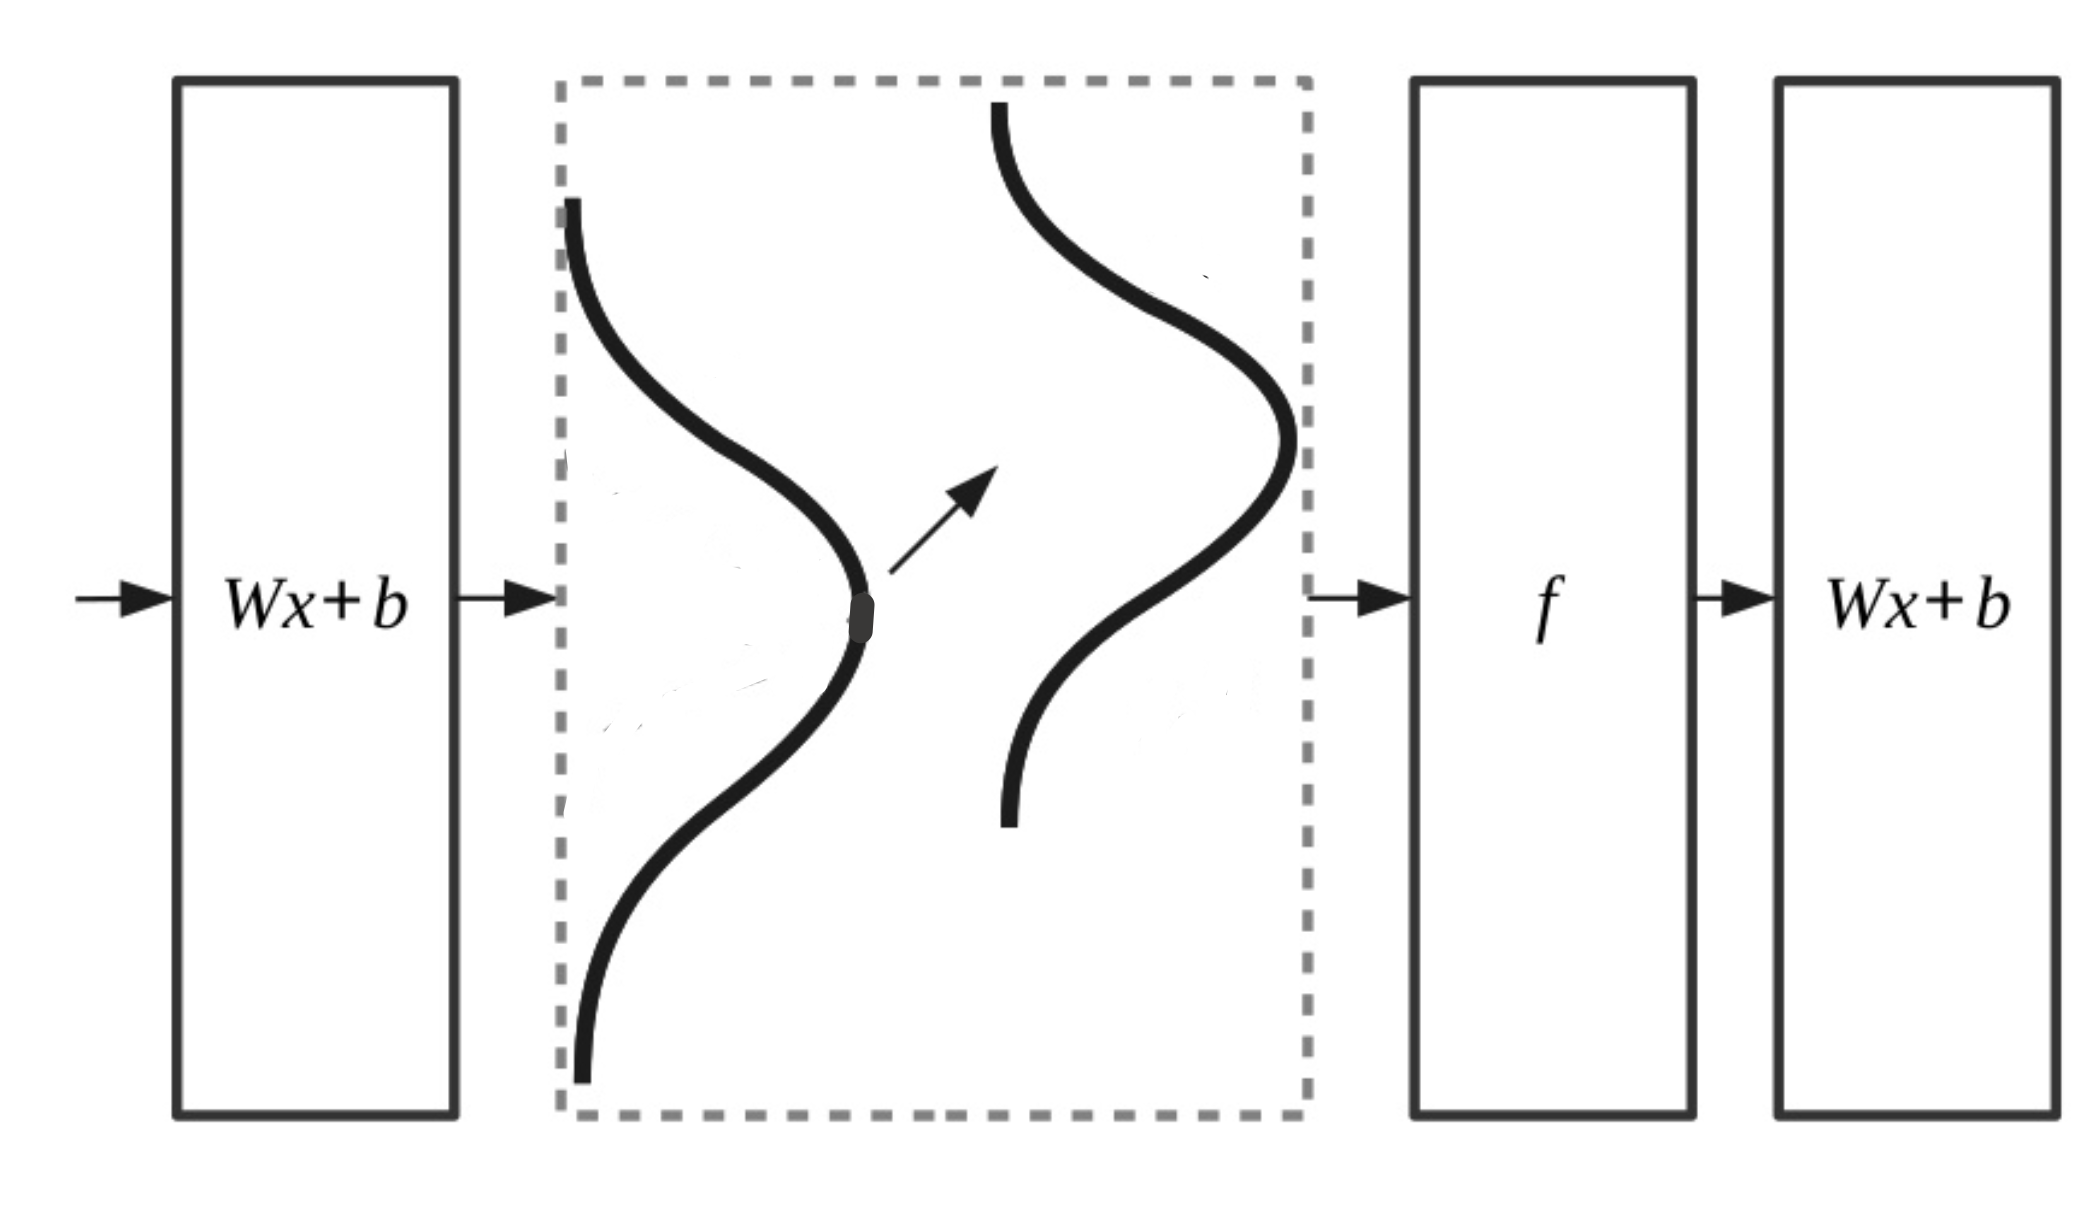
\includegraphics[width=.7\linewidth]{distributions_1.png}
	\end{center}
\end{frame}


\begin{frame}{А что внутри нейросетки?}
	\begin{center}
		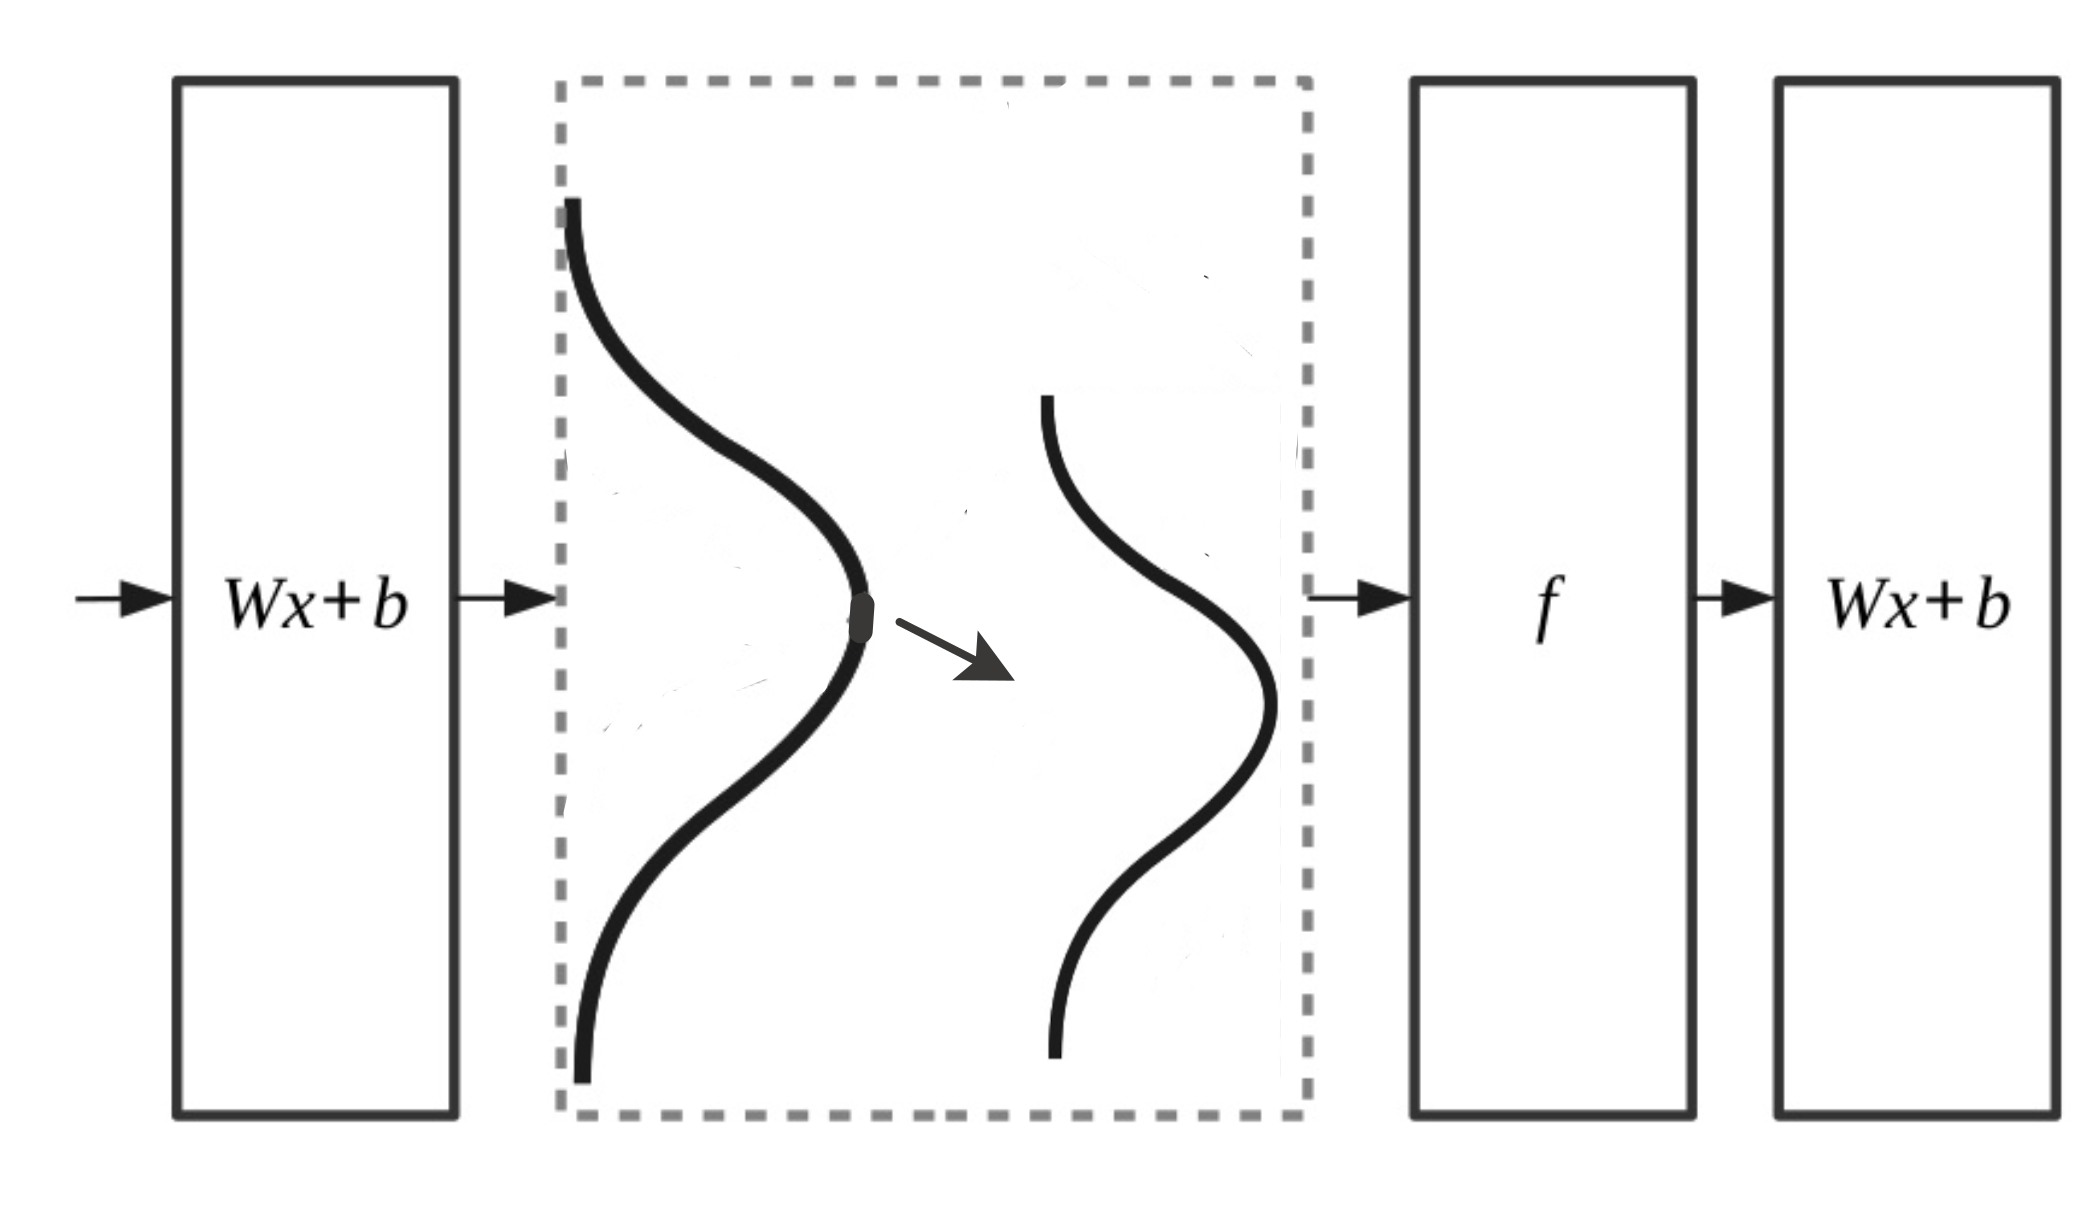
\includegraphics[width=.7\linewidth]{distributions_2.png}
	\end{center}
\end{frame}

\begin{frame}{Проблема}
	\begin{wideitemize}
		\item  Даже если мы стандартизовали вход $X$, внутри сетки может произойти несчастье и скрытый слой окажется нестандартизован 
		
	   \item  Скрытые представления $h = f(XW)$  могут менять своё распределение в процессе обучения, это усложняет его  
	   
	   	\item Давайте на каждом слое вместо $h$ использовать  $\hat{h} = \frac{h - \hat{\mu}_h}{\hat{\sigma}_h}$
	   	
	   	\item На выход будем выдавать $\beta \cdot  \hat h + \gamma$, для того, чтобы у нас было больше свободы, параметры $\beta$ и $\gamma$ учим как параметры полносвязного слоя
	\end{wideitemize}
\end{frame}


\begin{frame}{Batch Normalization (2015)}
	\begin{center}
		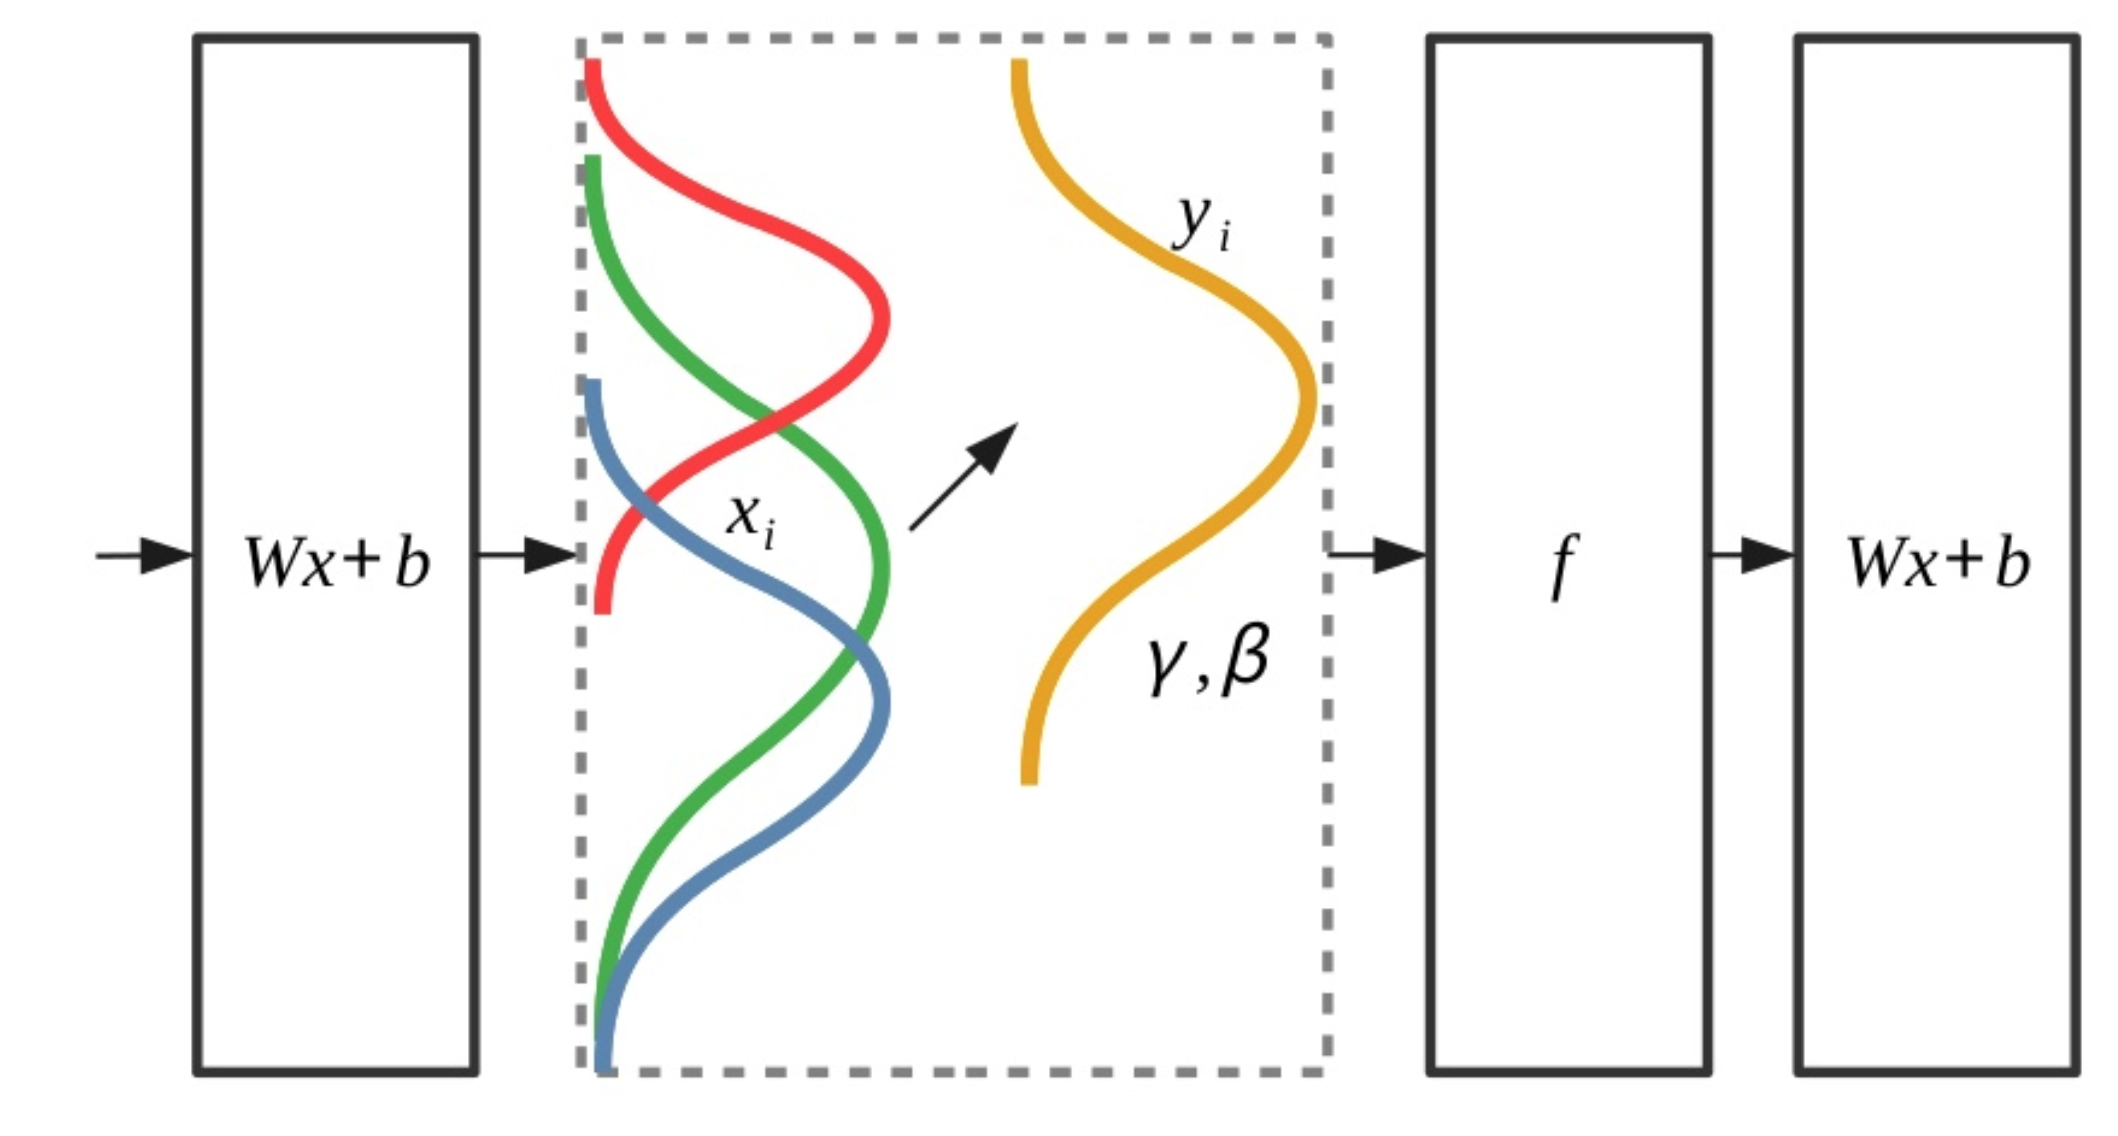
\includegraphics[width=.7\linewidth]{distributions_nice.png}
	\end{center}
\end{frame}


\begin{frame}{Forward pass}
	\begin{center}
		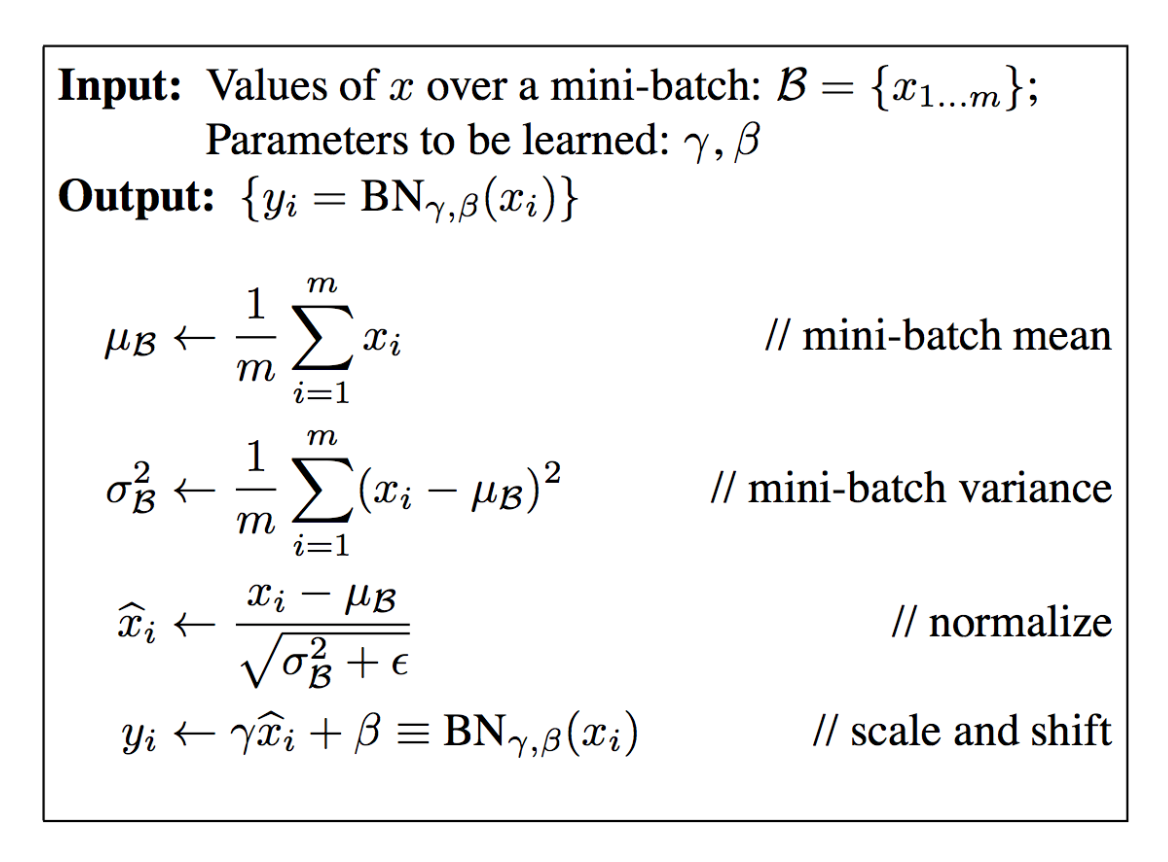
\includegraphics[width=.63\linewidth]{batch_formulas.png}
	\end{center}
	\vfill %
	\footnotesize
	{\color{blue} \url{https://arxiv.org/pdf/1502.03167.pdf}}
\end{frame}


\begin{frame}{Backward pass}
	\begin{center}
		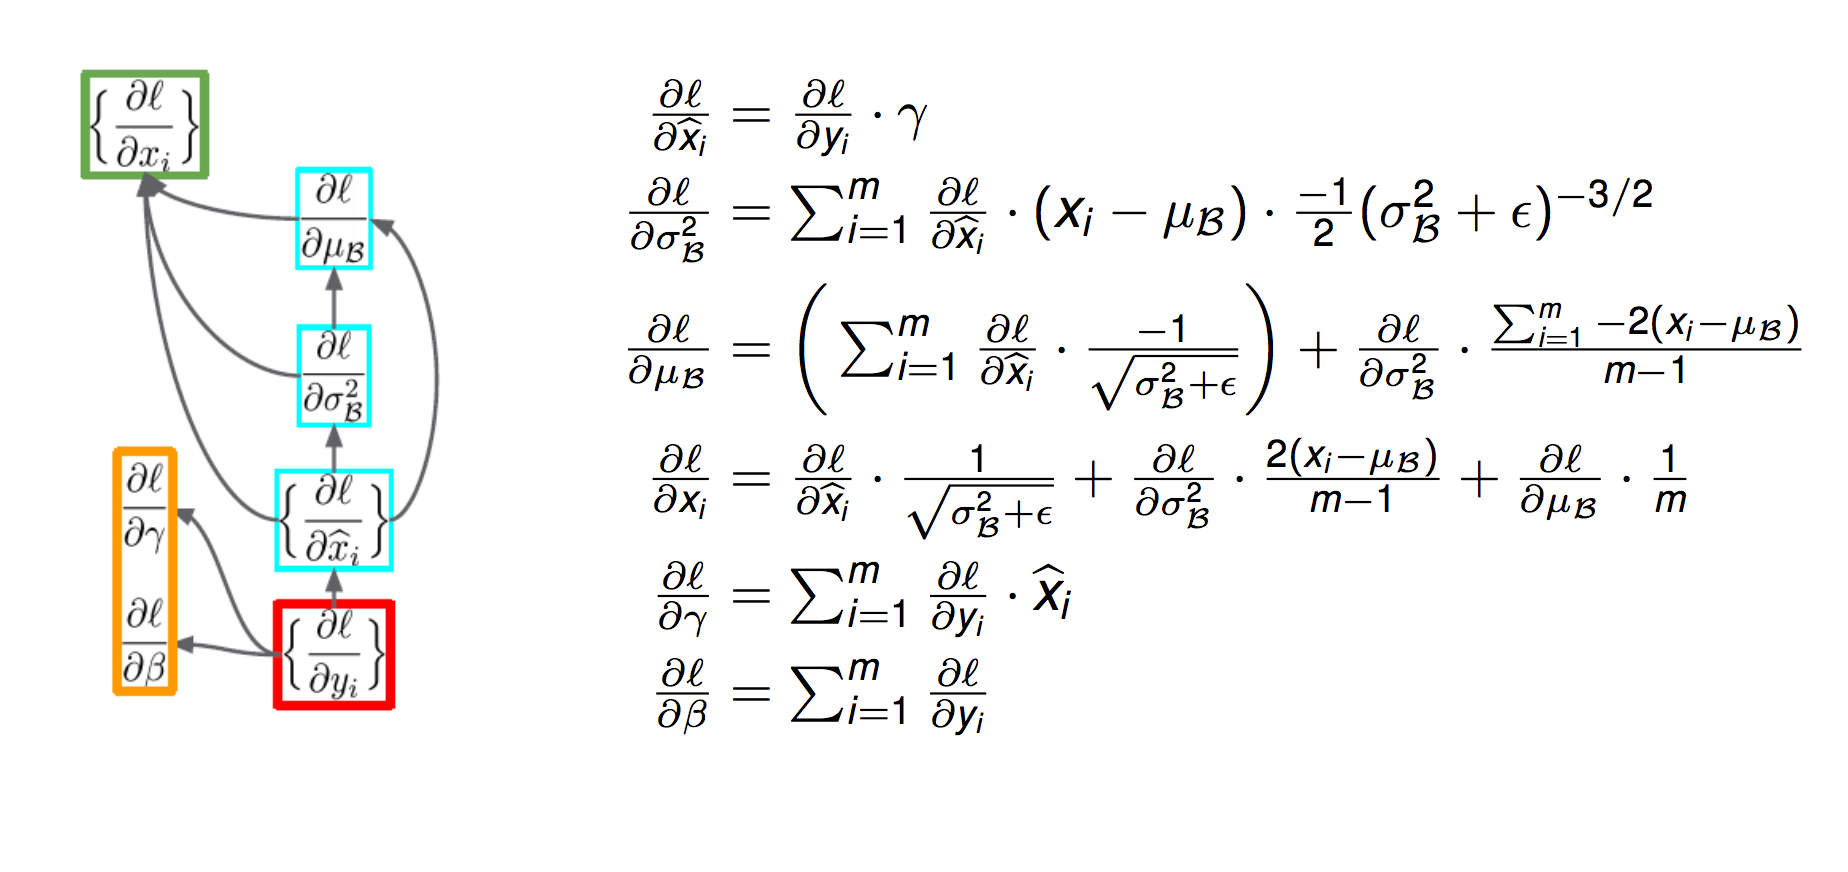
\includegraphics[width=.95\linewidth]{batch_grad.png}
	\end{center}
	\vfill %
	\footnotesize
	{\color{blue} \url{https://arxiv.org/pdf/1502.03167.pdf}}
\end{frame}


\begin{frame}{Batch Normalization (2015)}
	\begin{columns}[T] %
		\begin{column}{.3\textwidth}
			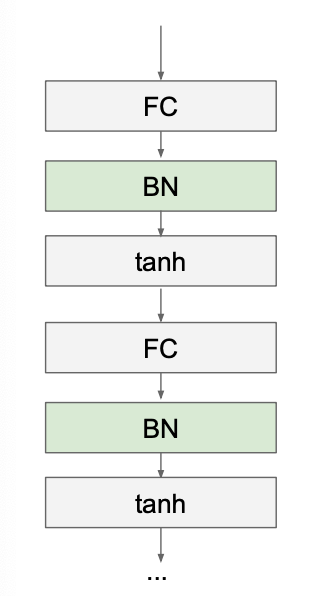
\includegraphics[width=.9\linewidth]{batch_norm_in_nn.png}
		\end{column}%
		\hfill%
		\begin{column}{.7\textwidth}
			\begin{wideitemize}
				\item  Делает обучение глубоких сетей проще
				\item Обеспечивает более высокие темпы обучения и более быструю сходимость
				\item Сети становятся более устойчивыми к инициализации
				\item Действует как регуляризатор во время обучения 
				\item \alert{Во время обучения и тестирования работает по-разному, это является источником большого числа багов и ошибок}
			\end{wideitemize}
		\end{column}%
\end{columns}
\end{frame}


\begin{frame}{Batch norm (2015)}
	\begin{wideitemize}
		\item  Как считать $\mu_h$ и $\sigma_h$? 
		
		\item Оценить по текущему батчу! 
		
		\begin{align*} 
			\mu_h =  \alpha \cdot \bar x_{batch}  + (1 - \alpha) \cdot \mu_h \\ 
			\sigma_h =  \alpha \cdot \hat s_{batch}  + (1 - \alpha) \cdot \sigma_h \\ 
		\end{align*}
		
		\item Коэффициенты $\beta$ и $\gamma$ оцениваются в ходе обратного распространения ошибки, $\mu$ и $\sigma$ не обучаются
		
		\item Обучение довольно сильно ускоряется, сходимость улучшается 
	\end{wideitemize}
	\vfill %
	\footnotesize
	{\color{blue} \url{https://arxiv.org/pdf/1502.03167.pdf}}
\end{frame}


\begin{frame}{Эксперимент с MNIST}
	\begin{center}
			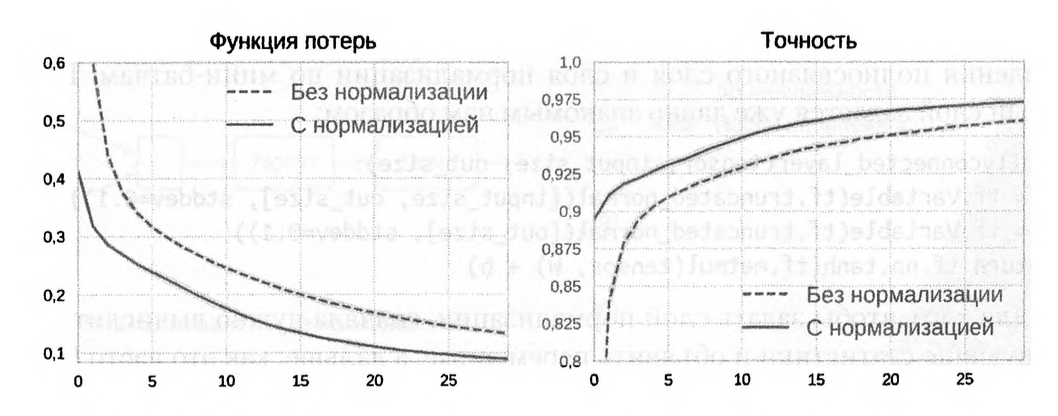
\includegraphics[width=.8\linewidth]{batch_norm.png}
		\end{center}
	\vfill
	{\small  Источник: Николенко, страница 160}
\end{frame}



% ToDo более адекватная картинка с экспериментами и возможно батч норм для сверток из презы стенфорда (84-86 слайды)


\begin{frame}{ Batch Normalization for convolutional networks}
\begin{center}
	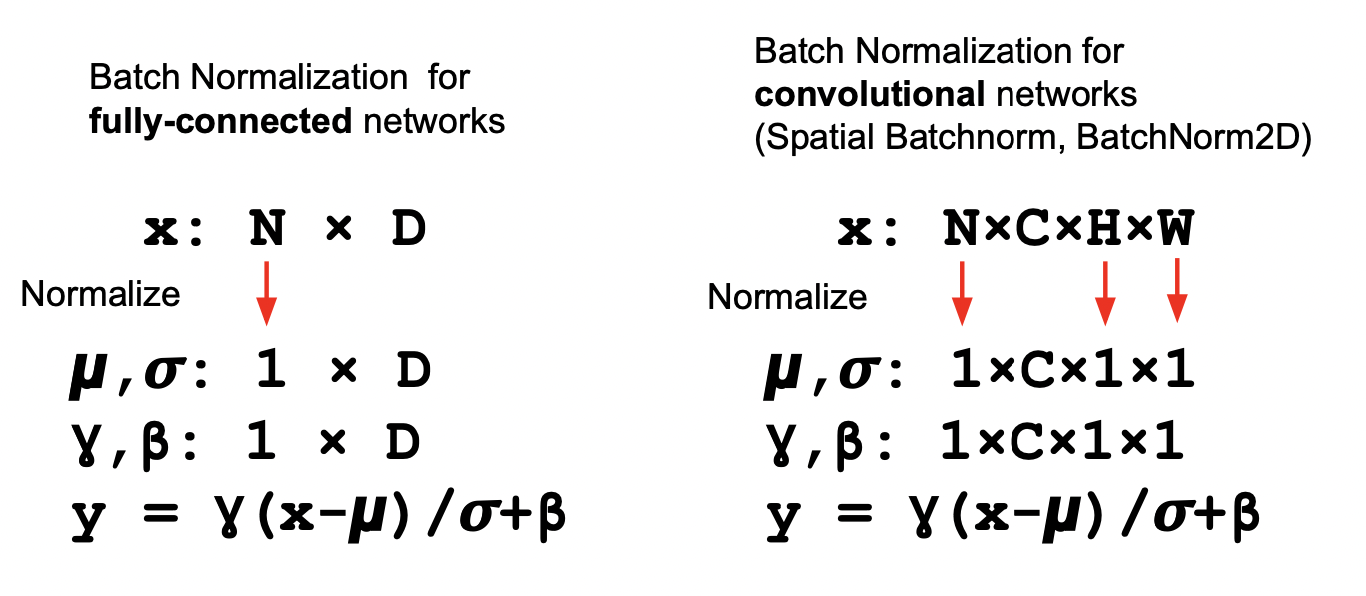
\includegraphics[width=.95\linewidth]{st_norm_1.png}
\end{center}
\vfill %
\footnotesize
Все скрины спёр у Стэнфорда, влом было набирать
\end{frame}



\begin{frame}{Layer Normalization (2016)}

\begin{center}
	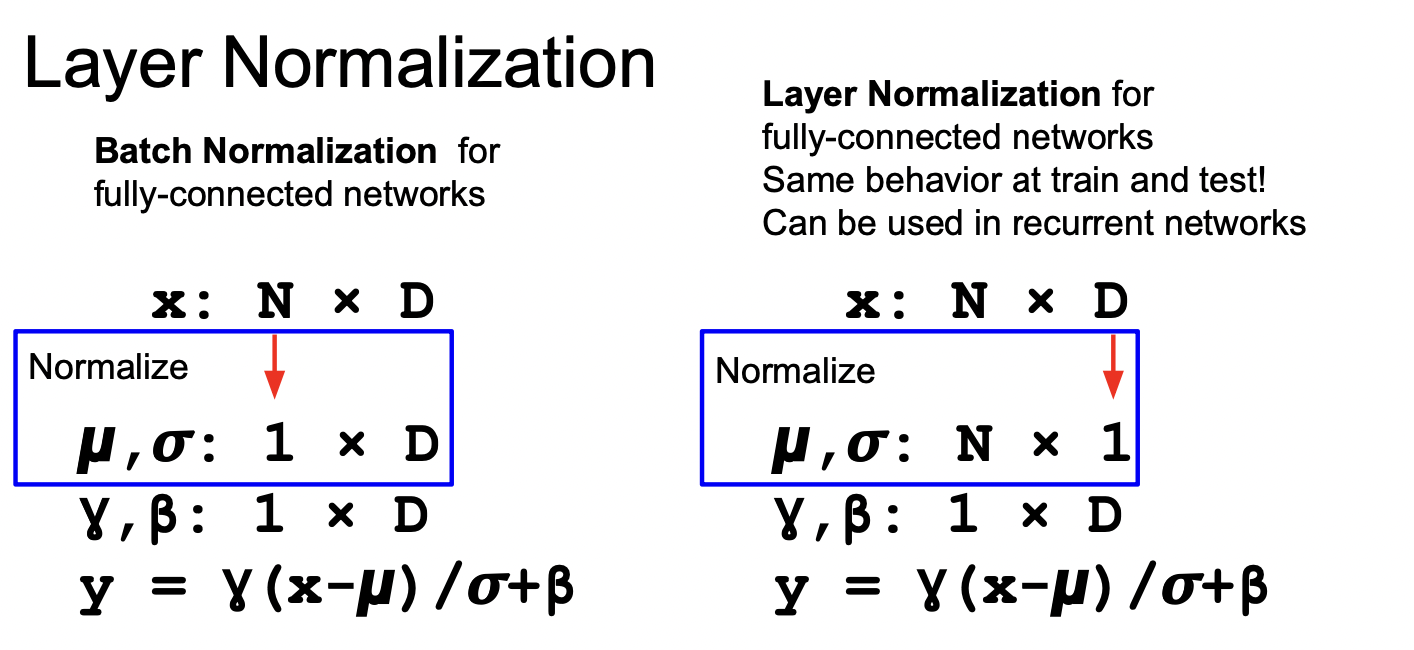
\includegraphics[width=.95\linewidth]{st_norm_2.png}
\end{center}
	\vfill %
\footnotesize
{\color{blue} \url{https://arxiv.org/pdf/1607.06450.pdf}}
\end{frame}


\begin{frame}{Instance Normalization (2017)}
\begin{center}
	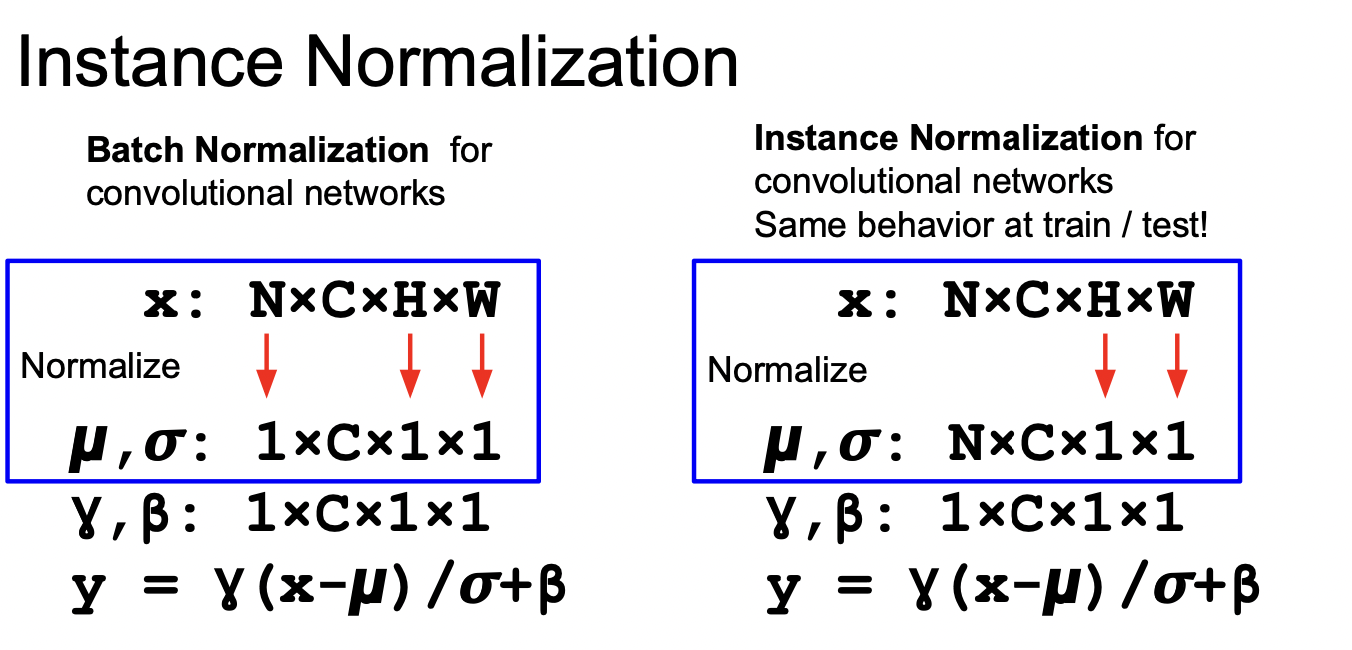
\includegraphics[width=.95\linewidth]{st_norm_3.png}
\end{center}
\end{frame}


\begin{frame}{Сравнение слоёв для нормализации}
\begin{center}
	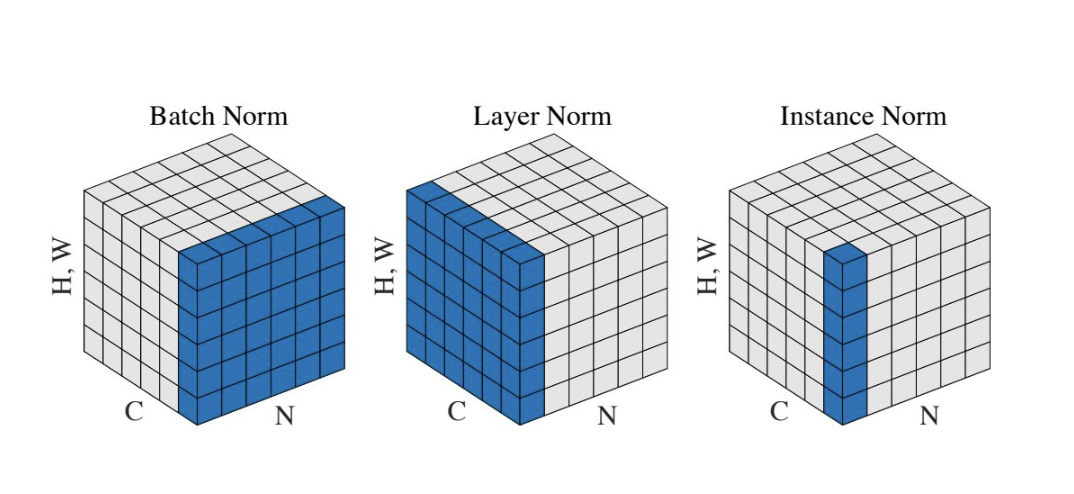
\includegraphics[width=.95\linewidth]{st_norm_4.png}
\end{center}
\end{frame}



\begin{frame}{Почему это помогает при обучении}
	\begin{center}
		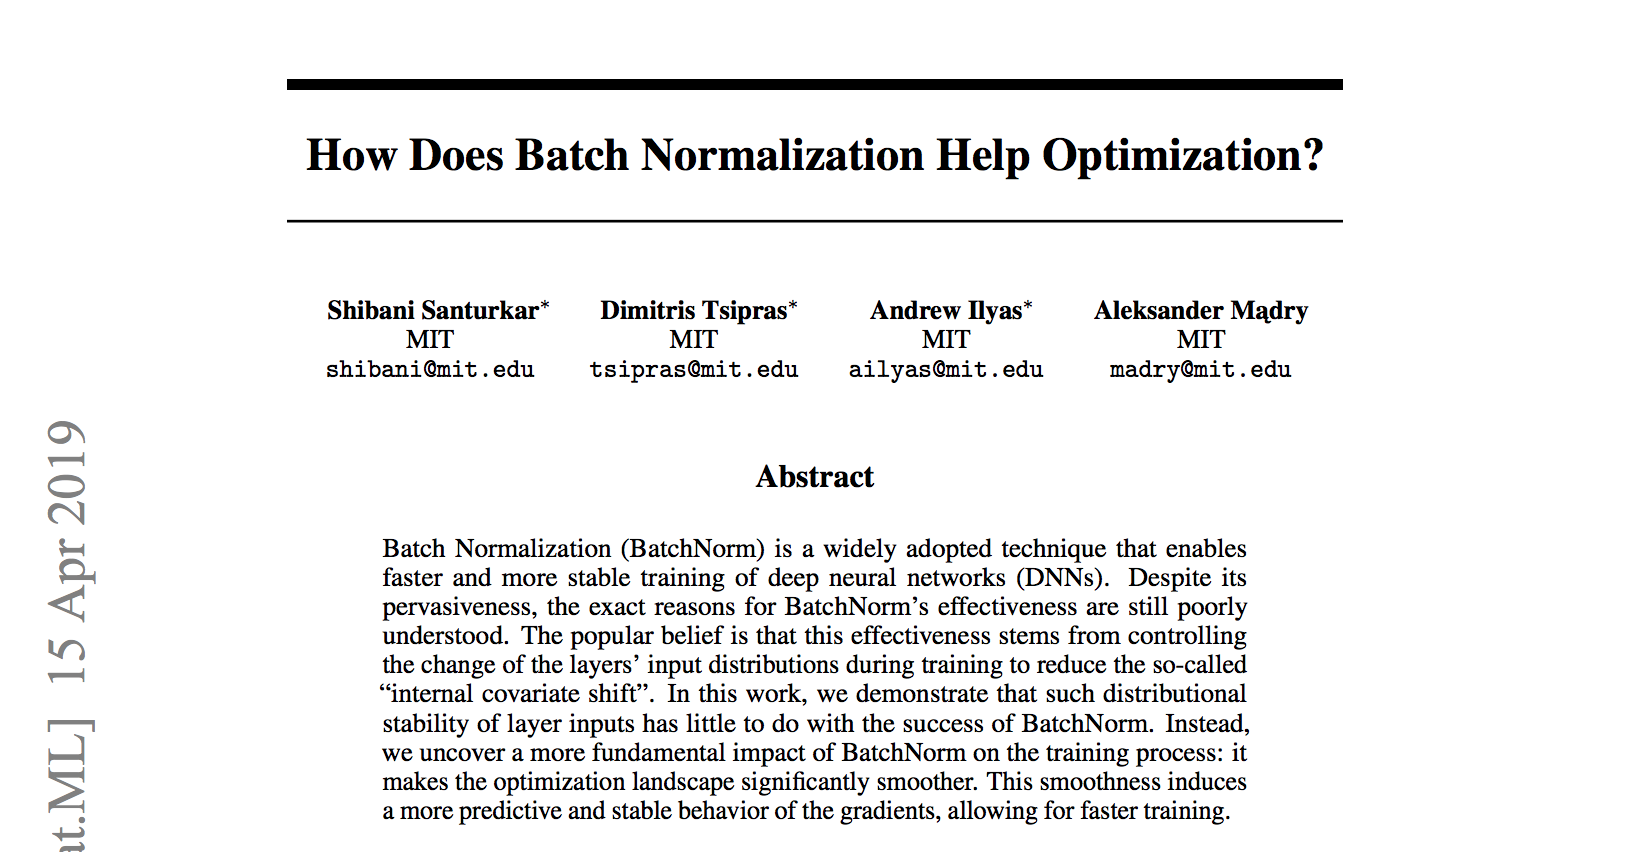
\includegraphics[width=.8\linewidth]{how_bn_help.png}
	\end{center}
	\vfill
	\footnotesize
	{\color{blue} \url{https://arxiv.org/abs/1805.11604}}
\end{frame}


\begin{frame}{Почему это помогает при обучении}
	\begin{center}
		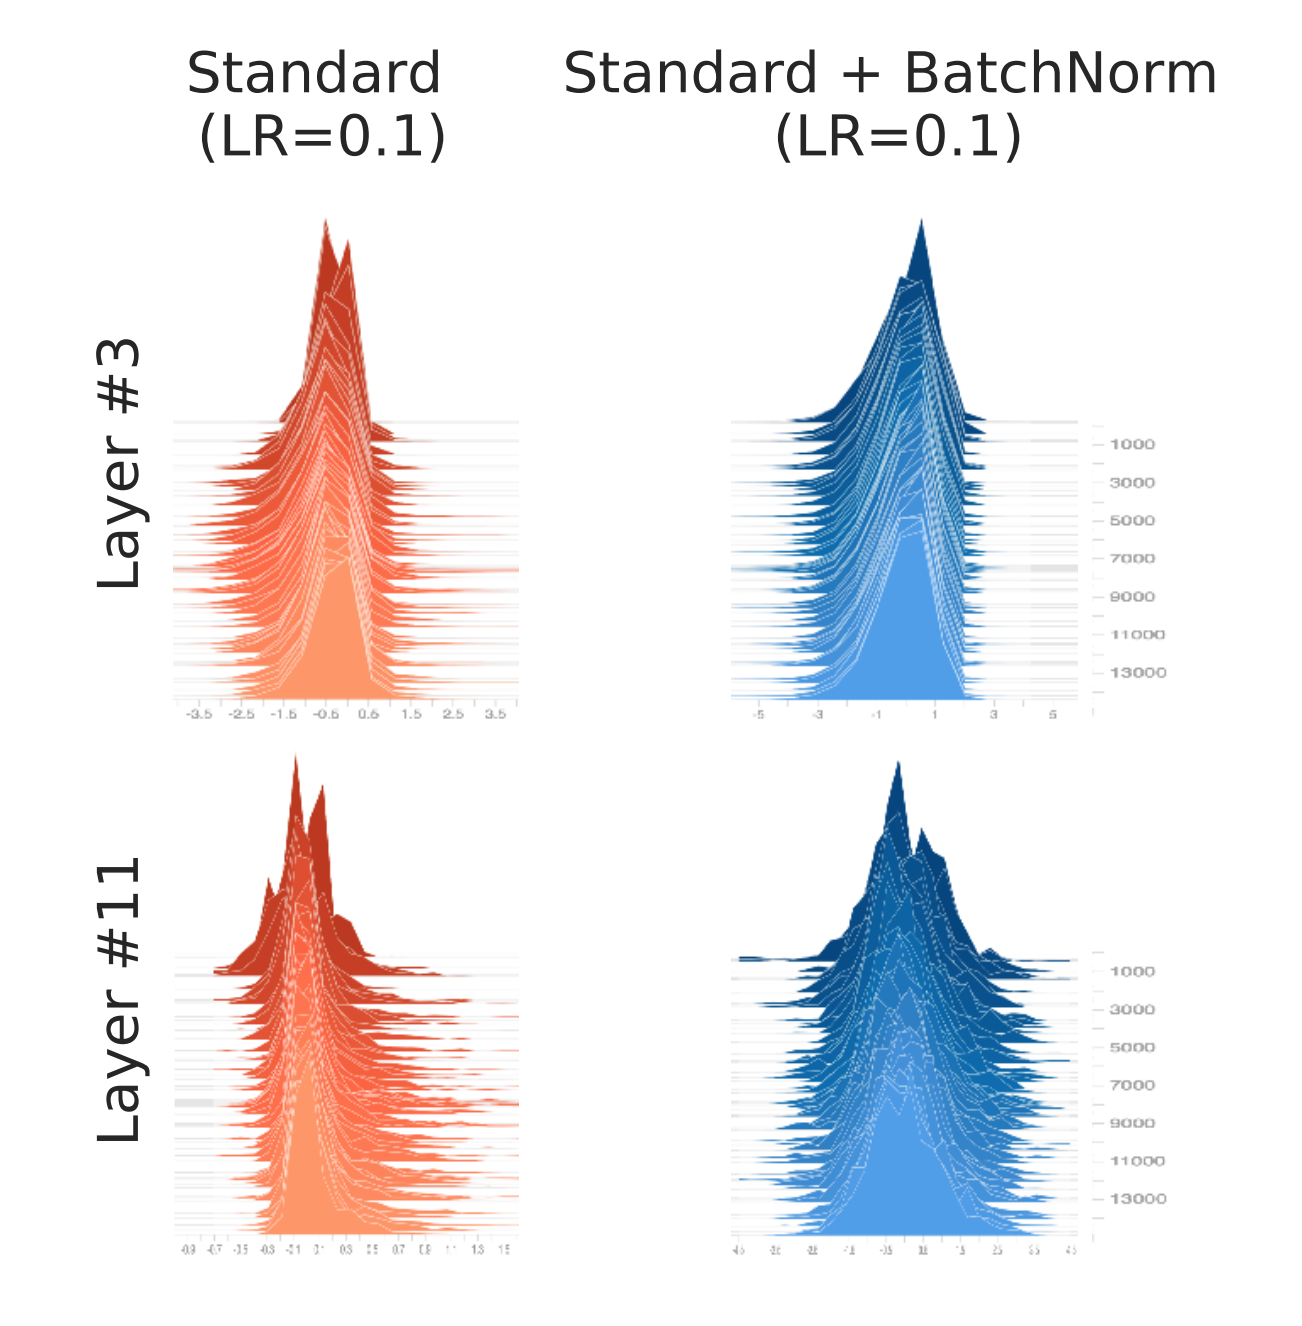
\includegraphics[width=.45\linewidth]{how_bn_help_2.png}
	\end{center}
	\vfill
	\footnotesize
	{\color{blue} \url{https://arxiv.org/abs/1805.11604}}
\end{frame}


\begin{frame}{Почему это помогает при обучении}
	\begin{center}
		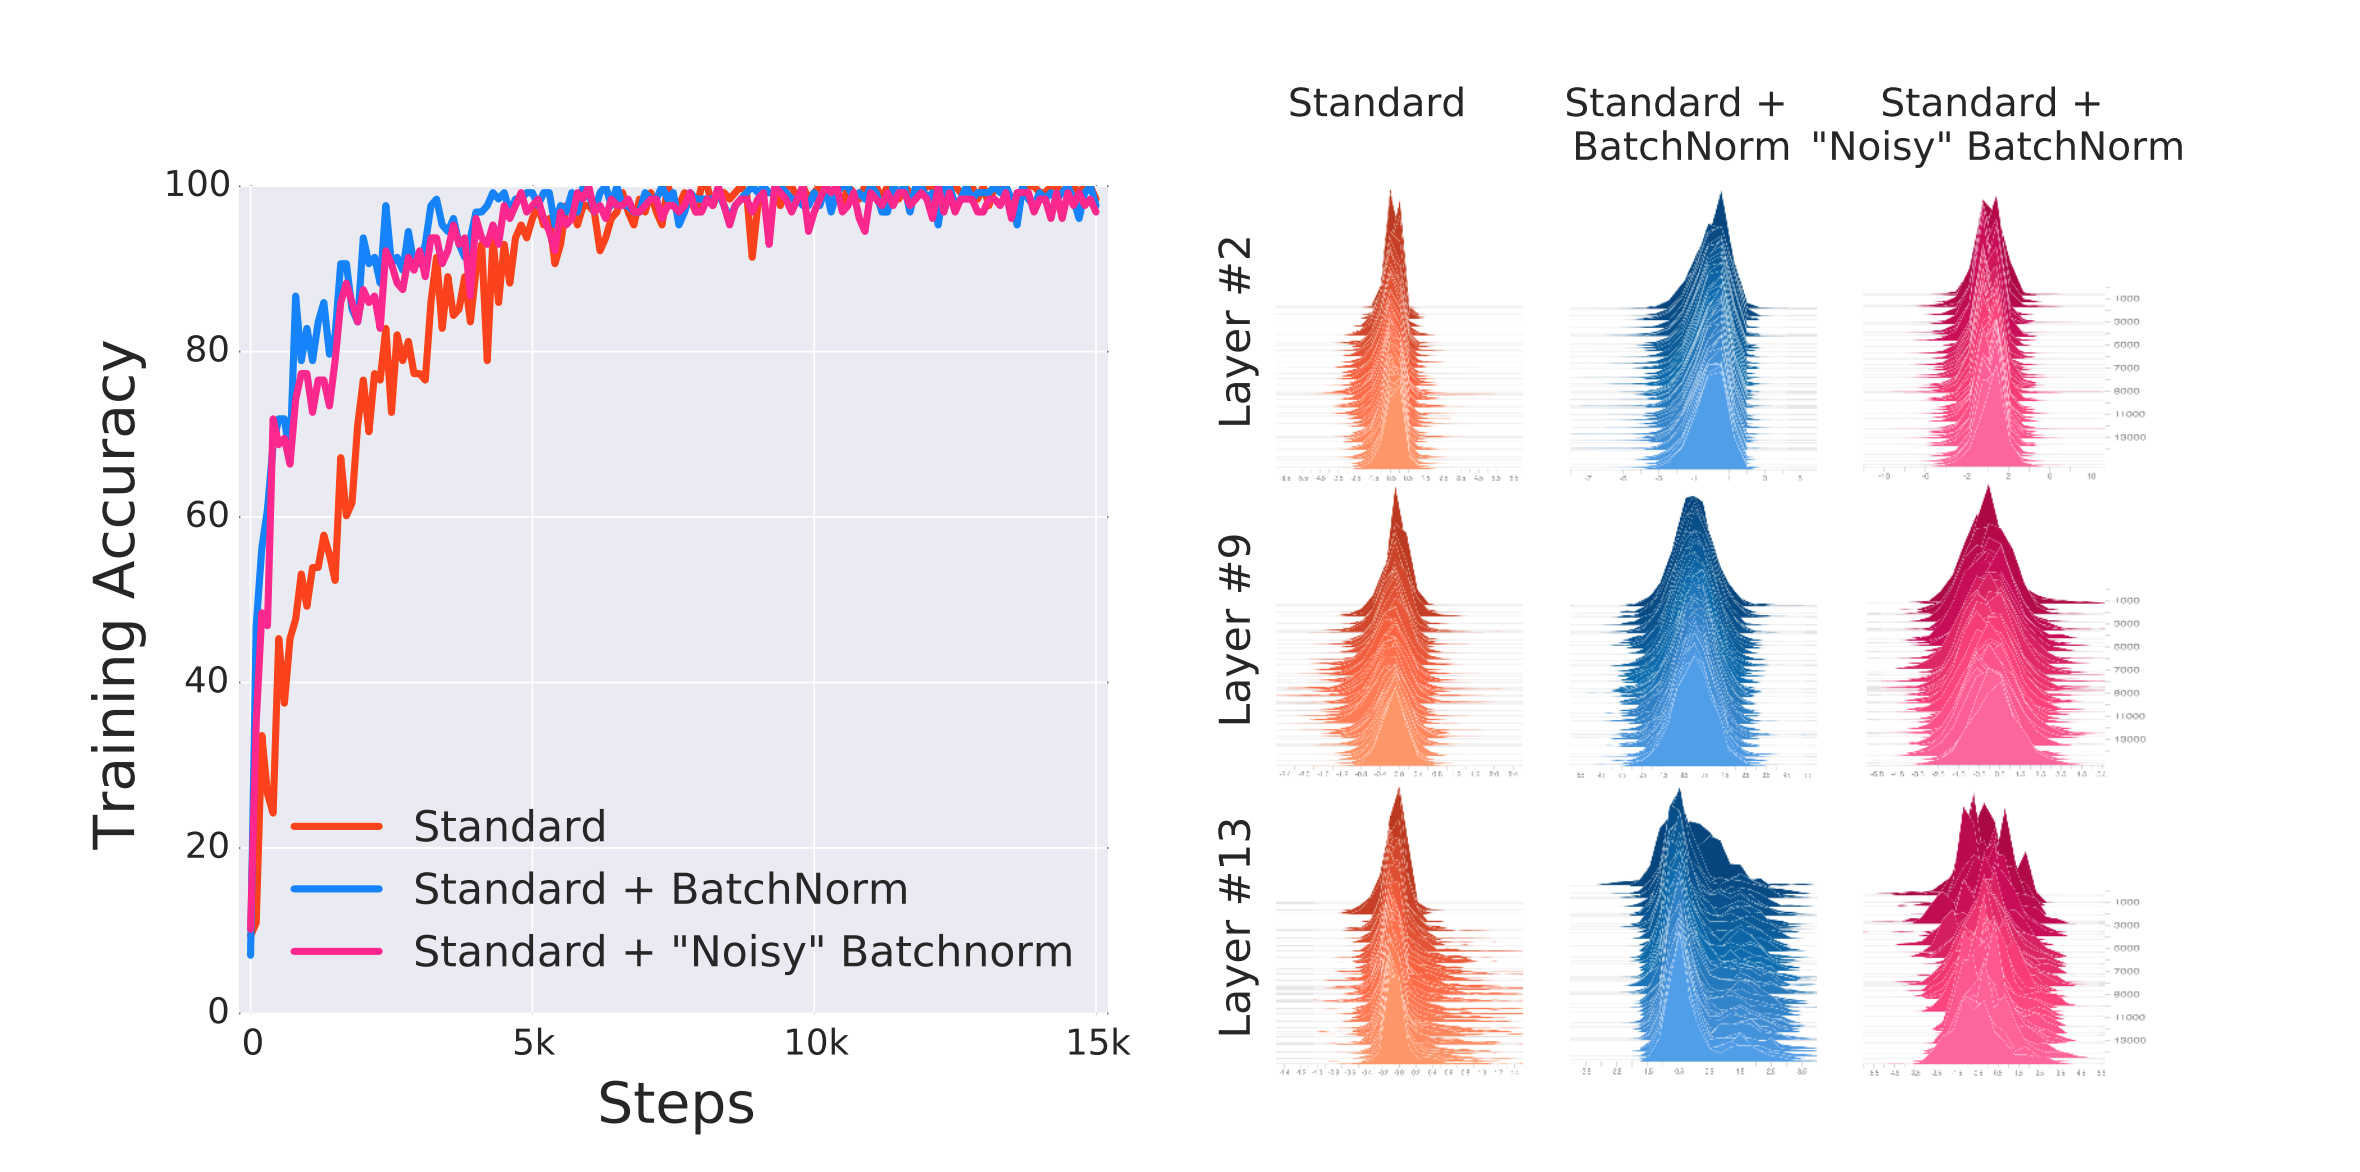
\includegraphics[width=.9\linewidth]{how_bn_help_3.png}
	\end{center}
	\vfill
	\footnotesize
	{\color{blue} \url{https://arxiv.org/abs/1805.11604}}
\end{frame}


\begin{frame}{Почему это помогает при обучении}
	\alert{Батчнорм сглаживает ландшафт функции потерь и из-за этого градиентный спуск идёт более гладко.}
	\begin{center}
		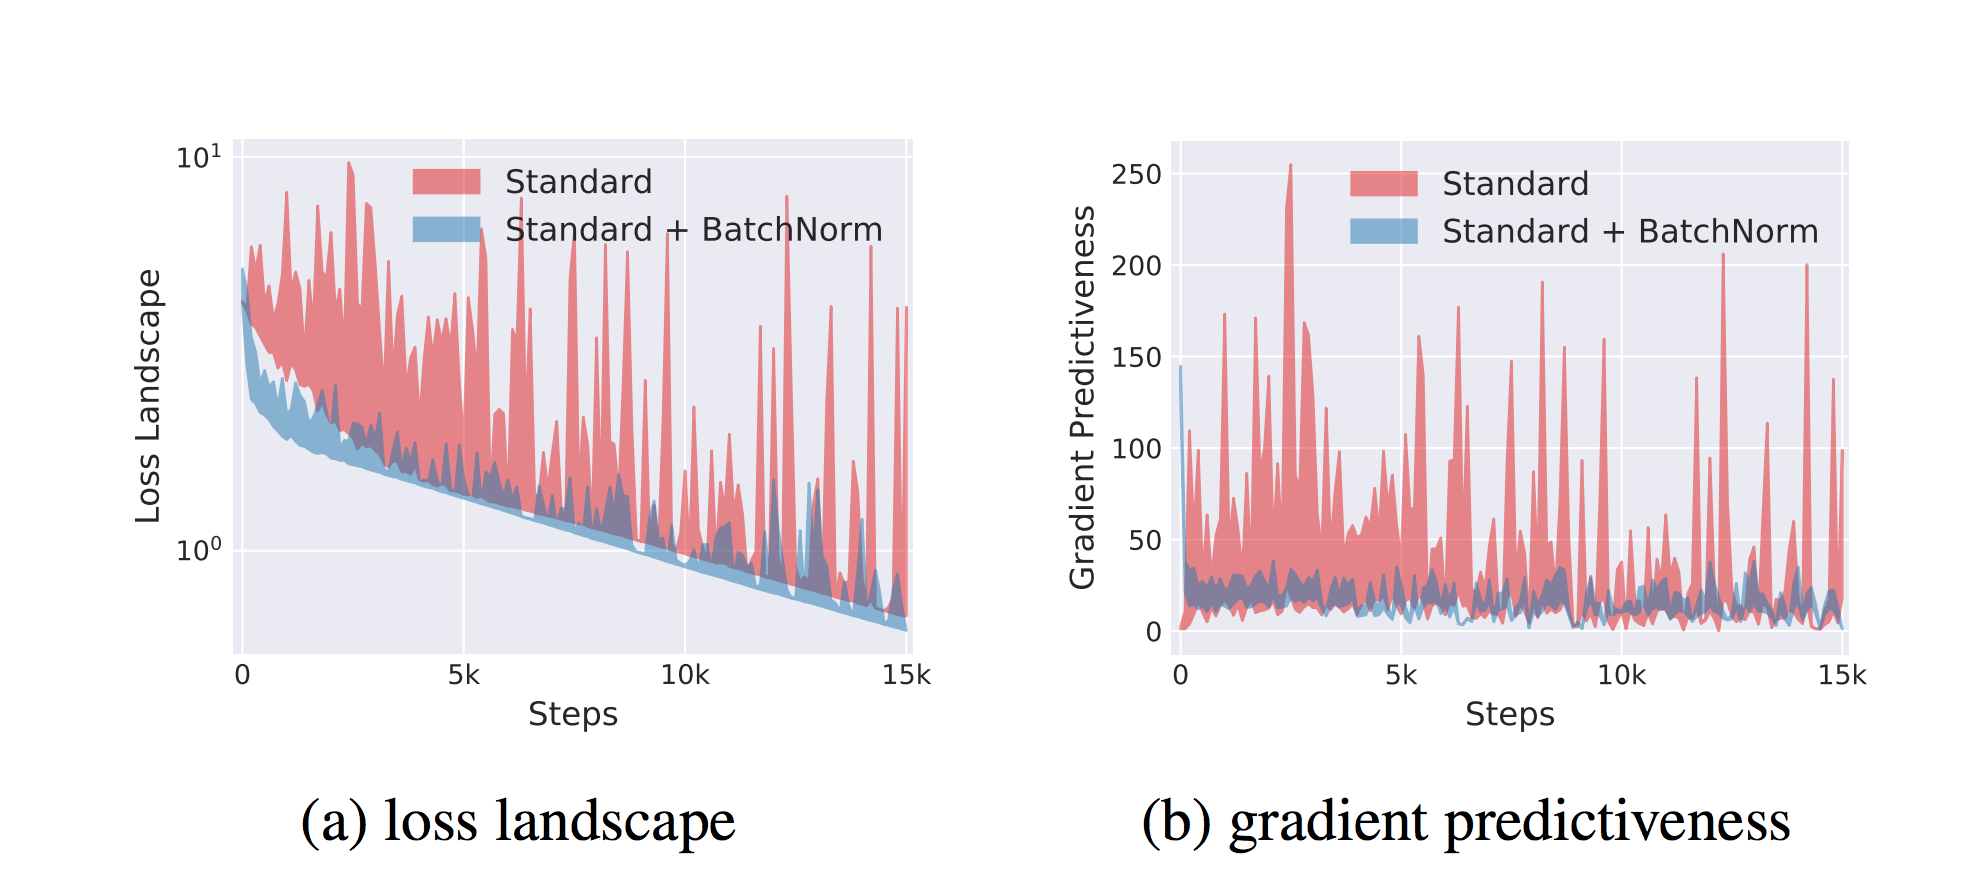
\includegraphics[width=.8\linewidth]{how_bn_help_4.png}
	\end{center}
	\vfill
	\footnotesize
	{\color{blue} \url{https://arxiv.org/abs/1805.11604}}
\end{frame}


\begin{frame}{Трюки}
	\begin{wideitemize}
		\item  С батч-нормализацией нужно уменьшить силу Dropout и регуляризацию
		
		\item Батч-нормализация и Dropout могут конфликтовать 
		
		\item  Не забывайте перемешивать обучающую выборку перед каждой новой эпохой, чтобы батчи были разнообразными 
		
		\item Существует довольно много техник нормализации:  Layer Normalization, Weight Normalization, Batch Renormalization, Adaptive Instance Normalization, Group Normalization etc.	
	\end{wideitemize}
	\vspace{3cm} %
	\footnotesize
	{\color{blue} \url{http://openaccess.thecvf.com/content_CVPR_2019/papers/Li_Understanding_the_Disharmony_Between_Dropout_and_Batch_Normalization_by_Variance_CVPR_2019_paper.pdf}}
\end{frame}




\begin{transitionframe}
	\begin{center}
		\Huge  Организация DL-экспериментов
	\end{center}
\end{transitionframe}


\begin{frame}{Проблемы при обучении нейросетей}
\begin{wideitemize}
	\item  «Neural net training is a leaky abstraction» — Andrej Karpathy
	\item  Знания архитектур, оптимизаторов порой недостаточно для получения хорошей модели
	\item Универсально наилучшего решения не бывает
	\item Важна точка начала экспериментов и инкрементальные улучшения
\end{wideitemize}
\vfill
\footnotesize
{\color{blue} \url{http://karpathy.github.io/2019/04/25/recipe/} \newline Максим Рябинин: \url{https://github.com/aosokin/dl_cshse_ami/blob/master/2021-fall/lectures/DL21-fall-lecture5-bestpractices.pdf} }
\end{frame}


\begin{frame}{Перед началом}
	\begin{wideitemize}
		\item  Используйте проверенные временем стандарты
		\item  Вместо своих моделей — архитектуры из популярных публикаций  (ResNet в зрении, ELMo/Transformer в текстах)
		\item Adam со стандартным LR без расписания обойти нелегко
		\item Сложные функции потерь/аугментации лучше отложить
		\item Первые запуски на небольших датасетах, подвыборке или синтетике
	\end{wideitemize}
\end{frame}


\begin{frame}{Как искать ошибки}
	\begin{wideitemize}	
		\item Чтобы легче находить ошибки, снизьте число факторов влияния 
		
		\item  Баги могут быть как в определении и обучении модели, так и в проверке качества (даже в загрузке данных)
		
		\item В меньшем масштабе можно быстрее итерироваться и находить проблемы
		
		\item \alert{Пробуйте прогнать код на одном батче и оценить, насколько адекватные результаты вы получили:} есть ли сходимость, есть ли переобучение на валидации, адекватно ли меняются метрики 
		
		\item Визуализируйте всё, что можете: метрики, примеры работы модели
		
		\item DL-код — всё ещё код: полезно писать unit-тесты
	\end{wideitemize}
\end{frame}



\begin{frame}{Типичные ошибки: модели}
\begin{wideitemize}
	\item Использование ad-hoc архитектур, когда не надо
	\item Использование нестабильных/сложных функций потерь вместо кросс-энтропии в классификации 
	\item Использование устаревших функций активации в глубоких сетях (сигмоид, тангенс)
	\item Плохая инициализация: нули/константы вместо Glorot/He
\end{wideitemize}
\end{frame}


\begin{frame}{Типичные ошибки: данные}
\begin{wideitemize}
	\item Отсутствие аугментации/использование некорректной аугментации, разные аугментации при обучении и валидации 
	\item Если используете предобученные модели, препроцессинг данных должен быть максимально похожим 
	\item Считывать все данные сразу, используйте Dataset 
\end{wideitemize}
\end{frame}


\begin{frame}{Типичные ошибки: обучение}
	\begin{wideitemize}
		\item Делайте чекпойнты, при них сохраняйте также параметры оптимизатора
		\item Функция потерь должна быть максимально близка к метрике, которую вы оптимизируете 
		\item Если используете pytorch, не забывайте делать \textit{zero\_grad} 
	\end{wideitemize}
\end{frame}


% Посмотреть готовые инструменты для логов: 
%  https://www.wandb.com/
% [2] https://www.comet.ml/
% [3] https://neptune.ai/ 
\begin{frame}{Организация экспериментов}
	\begin{wideitemize}
		\item \alert{Тестируйте за один раз только одно изменение,} чтобы понимать влияние каждого фактора по отдельности 
		\item На ранних стадиях не обязательно учить до сходимости и использовать всю выборку целиком
		\item  Ведите лог всех экспериментов
		\item Примеры инструментов для лога экспериентов:  \newline 
		\url{https://www.wandb.com/}  \newline 
		\url{https://www.comet.ml/}  \newline 
		\url{https://neptune.ai/}  \newline 
		\url{https://dvc.org/}  \newline 
		\url{https://mlflow.org/}  \newline 
	\end{wideitemize}

\end{frame}


\begin{frame}{Как улучшать качество?}
	\begin{wideitemize}
		\item Функция потерь должна быть максимально близка к метрике
		
		\item  Начните с небольших экспериментов и масштабируйтесь, когда всё отлажено 
		
		\item  \alert{Работа с данными (количество, качество, предобработка) зачастую приносит гораздо больше эффекта, чем перебор архитектур и оптимизаторов}
		
		\item  Архитектуры влияют существенно, но учитывайте свои ресурсы
		
		\item Занимайтесь оптимизацией гиперпараметров в самую последнюю очередь 
		
		\item Размер батча важен (ряд моделей иначе просто не учится)

	\end{wideitemize}
\end{frame}


\begin{frame}{Выводы}
	\begin{wideitemize}
		\item  Пользуйтесь проверенными техниками и опытом других людей
		
		\item  Начните с небольших экспериментов
		
		\item  Когда всё протестировано, можно масштабироваться
		
		\item  Отслеживайте все доступные метрики
		
		\item  Тестируйте одно изменение за раз
		
		\item  Сохраняйте код/конфигурацию всех экспериментов и их результаты
		
	\end{wideitemize}
\end{frame}




%%\begin{transitionframe}
%%	\begin{center}
%%		\Huge  Skip-connection и ResNet
%%	\end{center}
%%	\centering 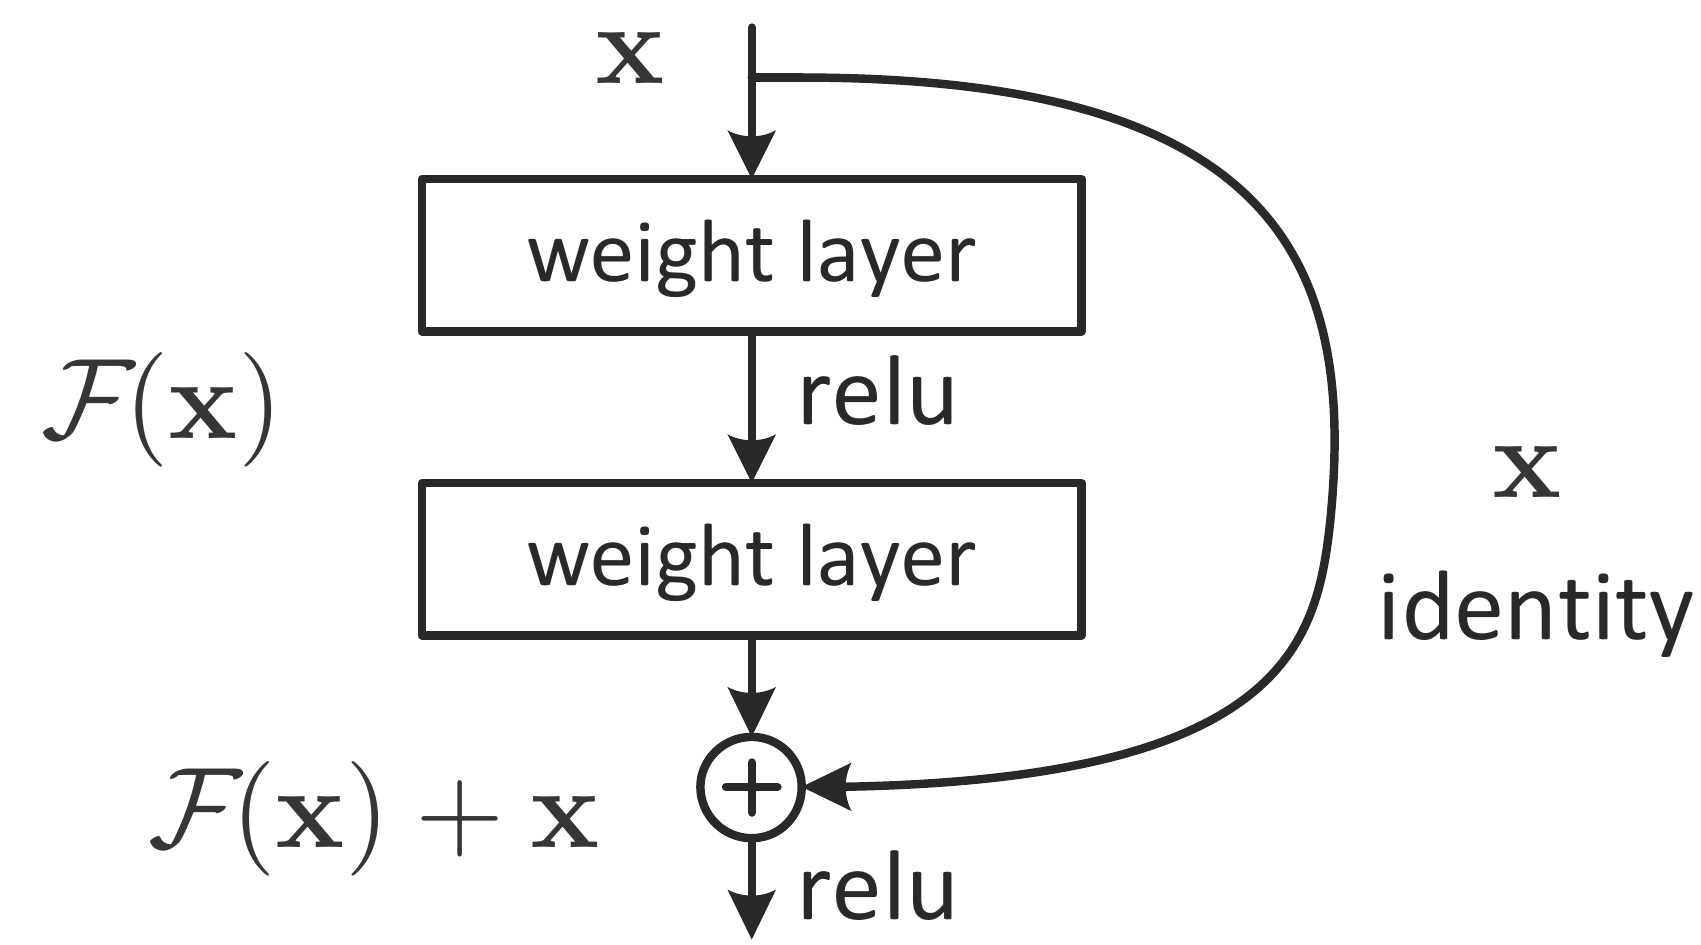
\includegraphics[scale = 0.1]{resnet_layer.png}
%%\end{transitionframe}
%%
%%\begin{frame}{Очень глубокие сети}
%%\begin{center}
%%	
\includegraphics[width=0.8\paperwidth]{we-need-to-go-deeper.jpg}
%%\end{center}
%%\end{frame}
%%
%%
%%\begin{frame}{Идея ResNet}
%%
%%Чем глубже нейронная сеть, тем сложнее её обучать, возникает новая проблема, которую нельзя свести к переобучению или затуханию градиента. \alert{Её называют деградация обучения (training degradation)}
%%
%%\begin{center}
%%	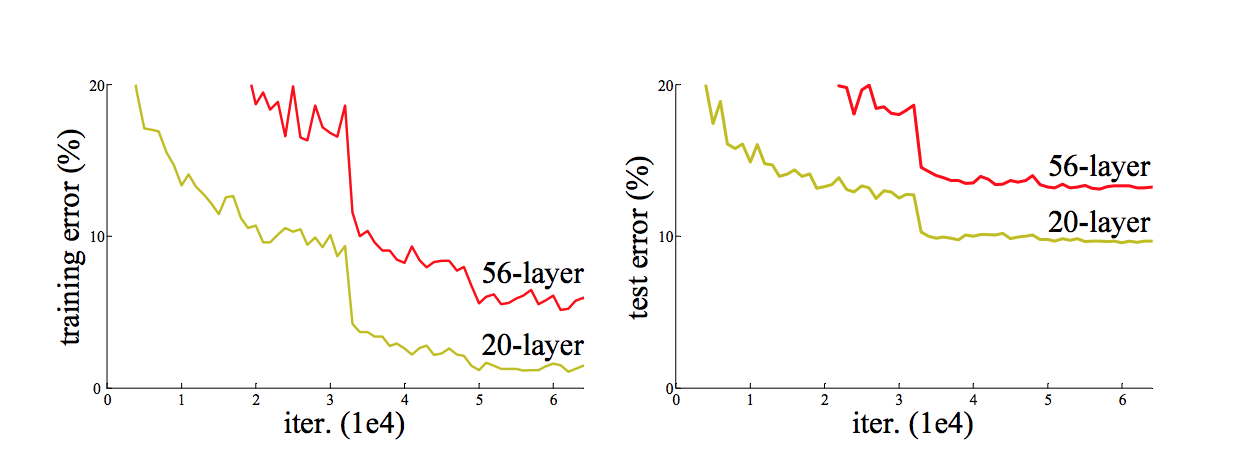
\includegraphics[width=0.8\paperwidth]{resnet_idea.png}
%%\end{center}
%%
%%\vfill %
%%\footnotesize
%%\color{blue} \url{https://arxiv.org/abs/1512.03385}
%%\end{frame}
%%
%%\begin{frame}{Идея ResNet}
%%\begin{wideitemize}
%%	\item  Огромная свёрточная сеть из $20$ слоёв и свёрточная сеть из $56$ слоёв,  большая сетка обучается хуже
%%	\item  \alert{Проблема:} слои инициализированы шумом, если какой-то один слой не натренирован, он убивает работу сети, через него не проходит полезный сигнал 
%%	\item Чем больше слоёв, тем более ярко выражен этот эффект 
%%	\item \alert{Решение:} Будем посылать вход на выход и давать слою возможность немного его подправить (residual слой)
%%	\item Идея чем-то похожа на бустинг, сеть сама решает когда заканчивать подправлять выходы (грубо говоря, сама выбирает глубину)
%%\end{wideitemize}
%%\end{frame}
%%
%%
%%\begin{frame}{ResNet (2015)}
%%\begin{center}
%%	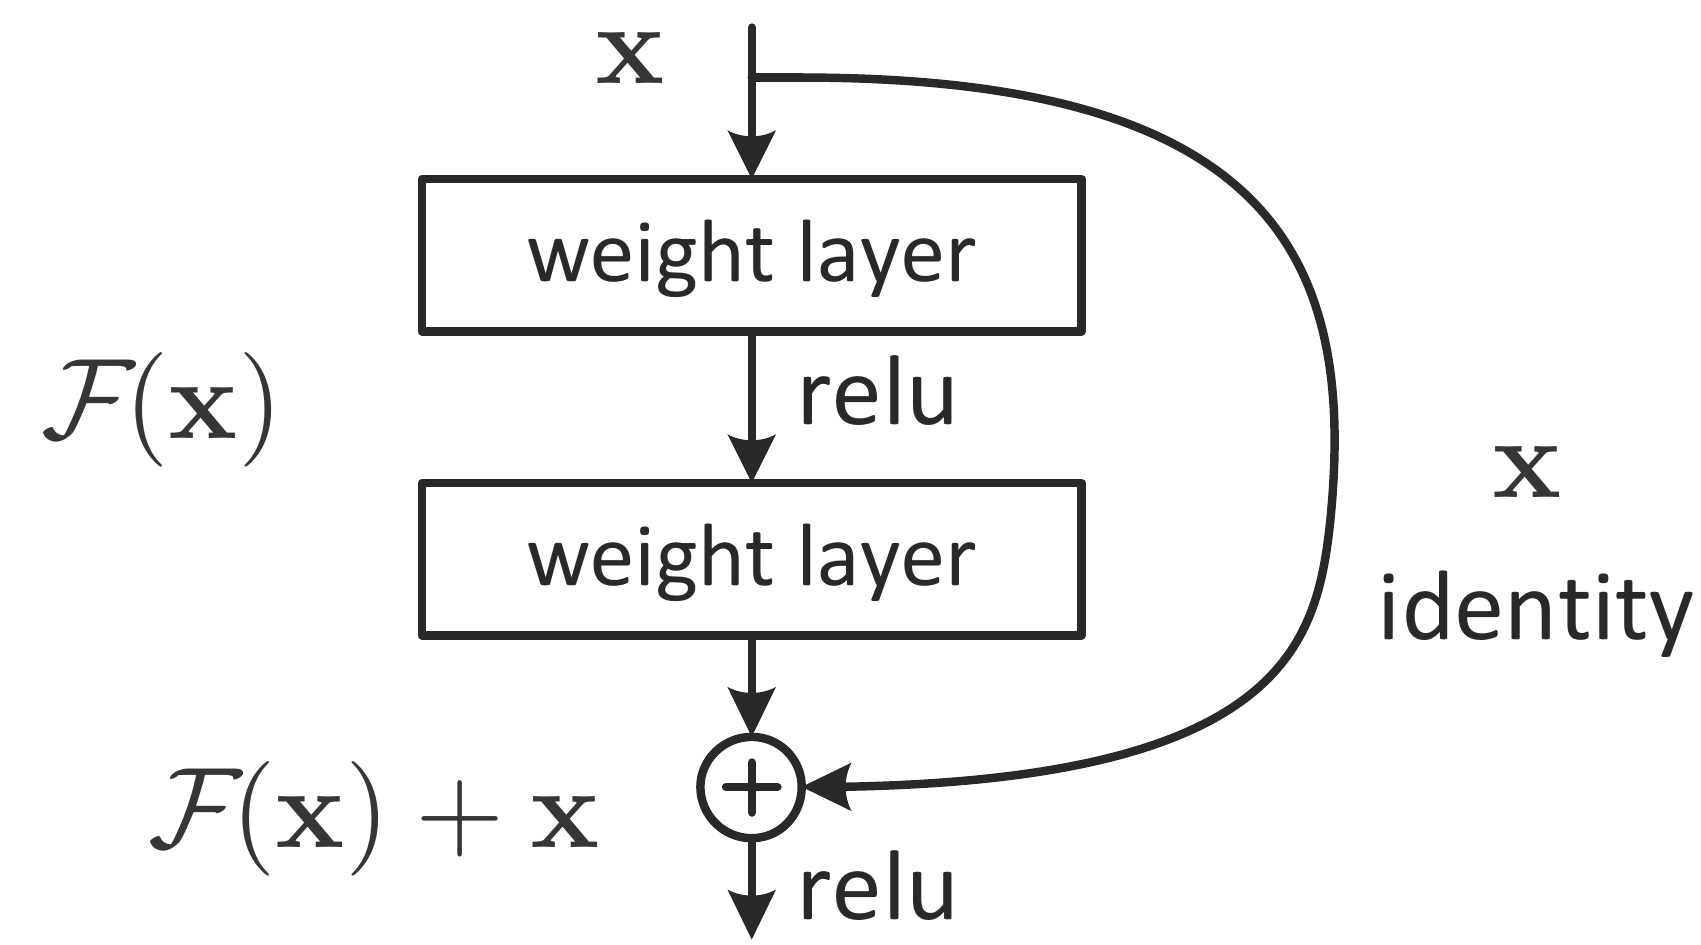
\includegraphics[scale=0.2]{resnet_layer.png}
%%\end{center}
%%\vfill %
%%\footnotesize
%%\color{blue} \url{https://arxiv.org/abs/1512.03385}
%%\end{frame}
%%
%%
%%\begin{frame}{ResNet (2015)}
%%\begin{center}
%%	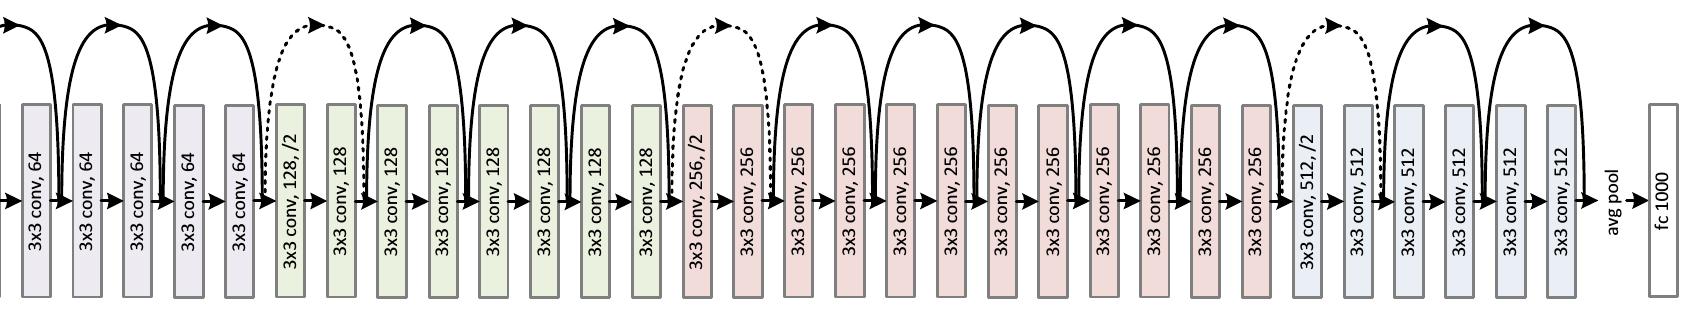
\includegraphics[width=0.8\paperwidth]{resnet.png}
%%\end{center}
%%\vfill %
%%\footnotesize
%%\color{blue} \url{https://arxiv.org/abs/1512.03385}
%%\end{frame}
%%
%%
%%\begin{frame}{ResNet (2015)}
%%\begin{wideitemize}
%%\item \alert{Идея:} более глубокие уровни должны улавливать разницу между новым и тем, что было раньше 
%%
%%\item Ключевым элементом архитектуры является связь, которая пропускает несколько слоёв, передавая результат предыдущего слоя
%%
%%\item Такое изменение позволило полностью отказаться от таких техник регуляризации, как DropOut
%%
%%\item Градиенты не взрываются, свойства ResNet активно пытаются сейчас изучать
%%
%%\item  ResNet-архитектура ведёт себя как ансамбль неглубоких сетей:  \color{blue} \url{https://arxiv.org/abs/1605.06431}
%%\end{wideitemize}
%%\end{frame}
%%
%%
%%\begin{frame}{Визуализация потерь}
%%\begin{center}
%%	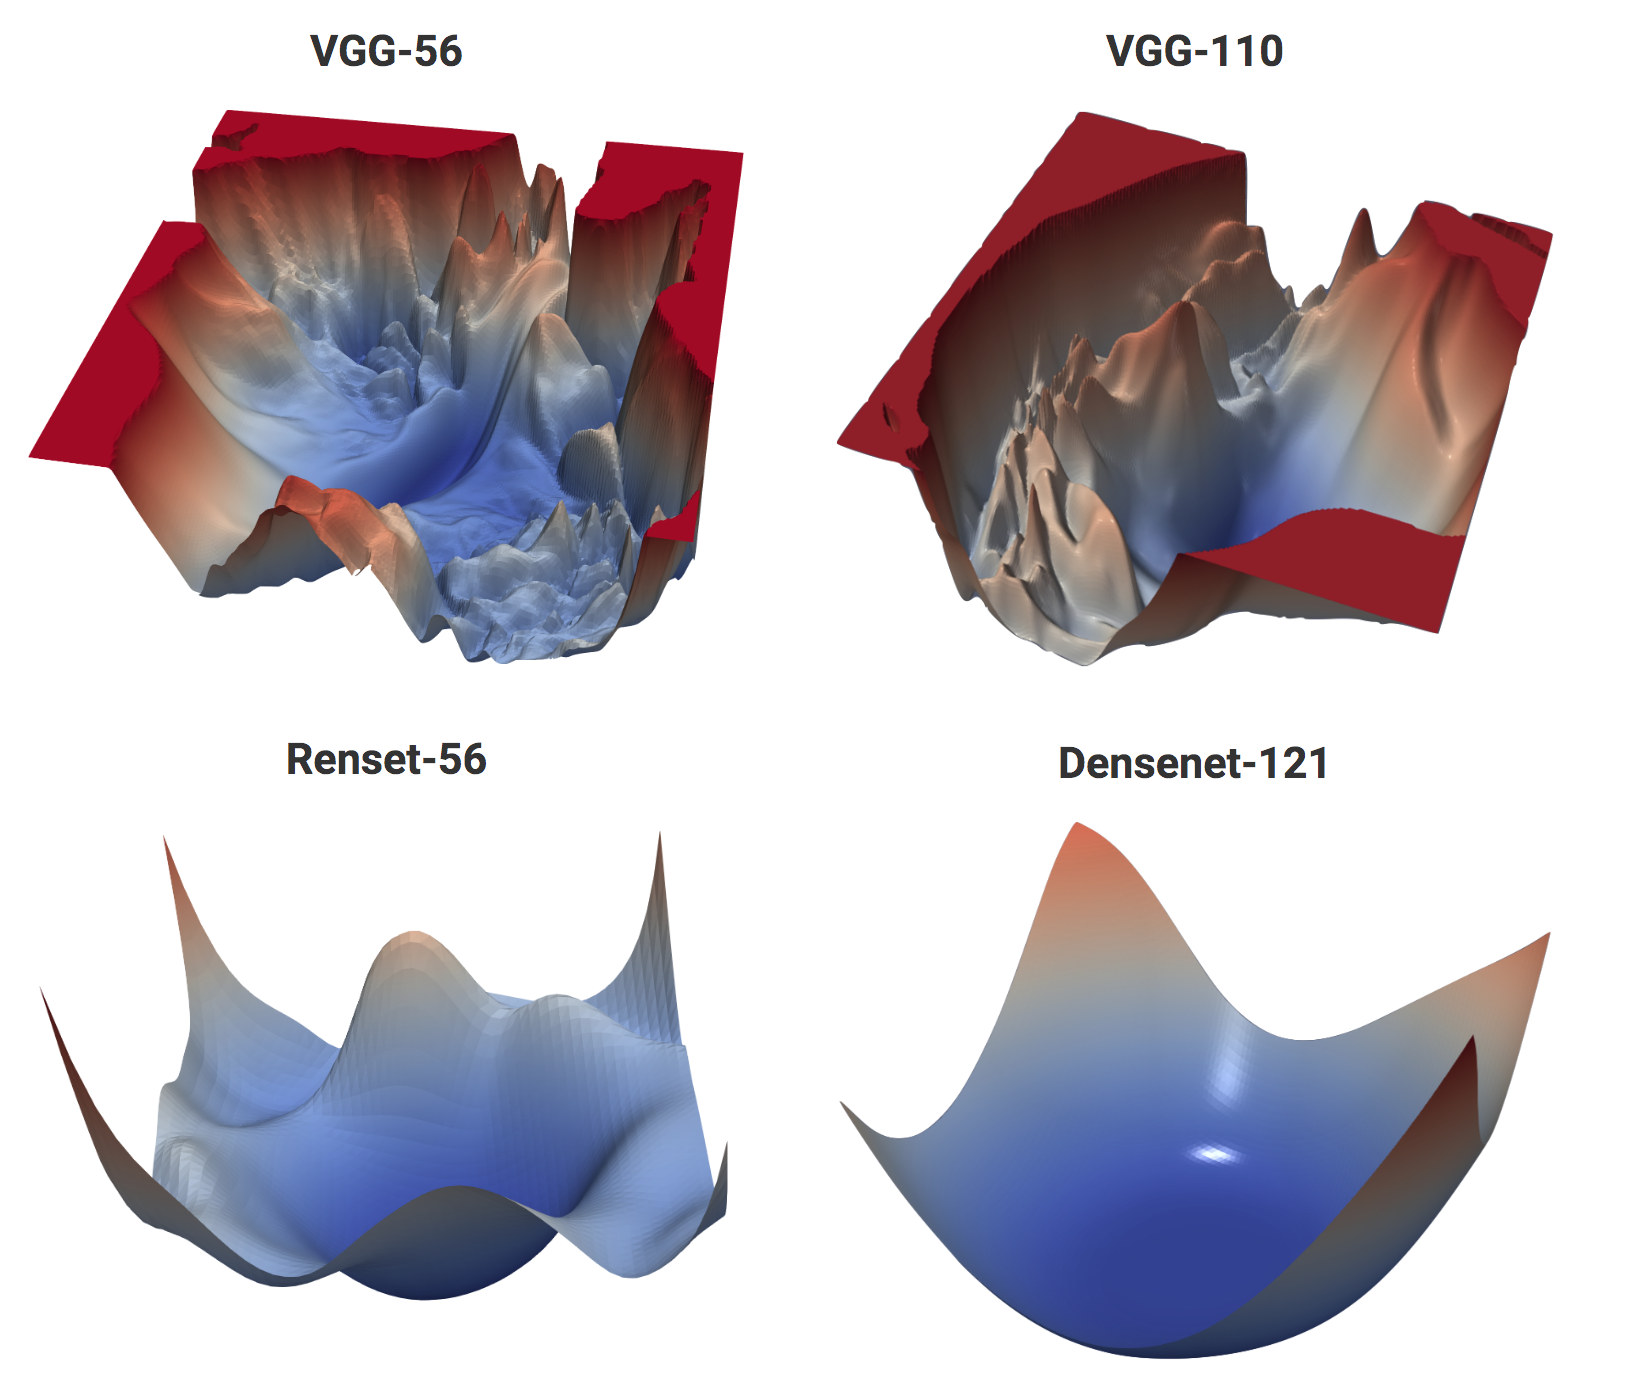
\includegraphics[width=0.5\paperwidth]{loss.png}
%%\end{center}
%%\vfill %
%%\footnotesize 
%%\color{blue} \url{https://arxiv.org/pdf/1712.09913.pdf} \newline  \url{https://github.com/tomgoldstein/loss-landscape}
%%\end{frame}
%%
%%
%%\begin{frame}{ResNet}
%%\begin{wideitemize}
%%	\item  ResNet породил целый букет новых архитектур
%%	
%%	\item Сегодня эта идея активно используется в рекурентных сетках и трансформерах 
%%\end{wideitemize}
%%\end{frame}


%%\begin{transitionframe}
%%	\begin{center}
%%		\Huge  Нейросети со стохастической глубиной
%%	\end{center}
%%	\centering 
\includegraphics[scale = 0.1]{deep.png}
%%\end{transitionframe}
%%
%%
%%\begin{frame}{Нейросети со стохастической глубиной}
%%\begin{center}
%%	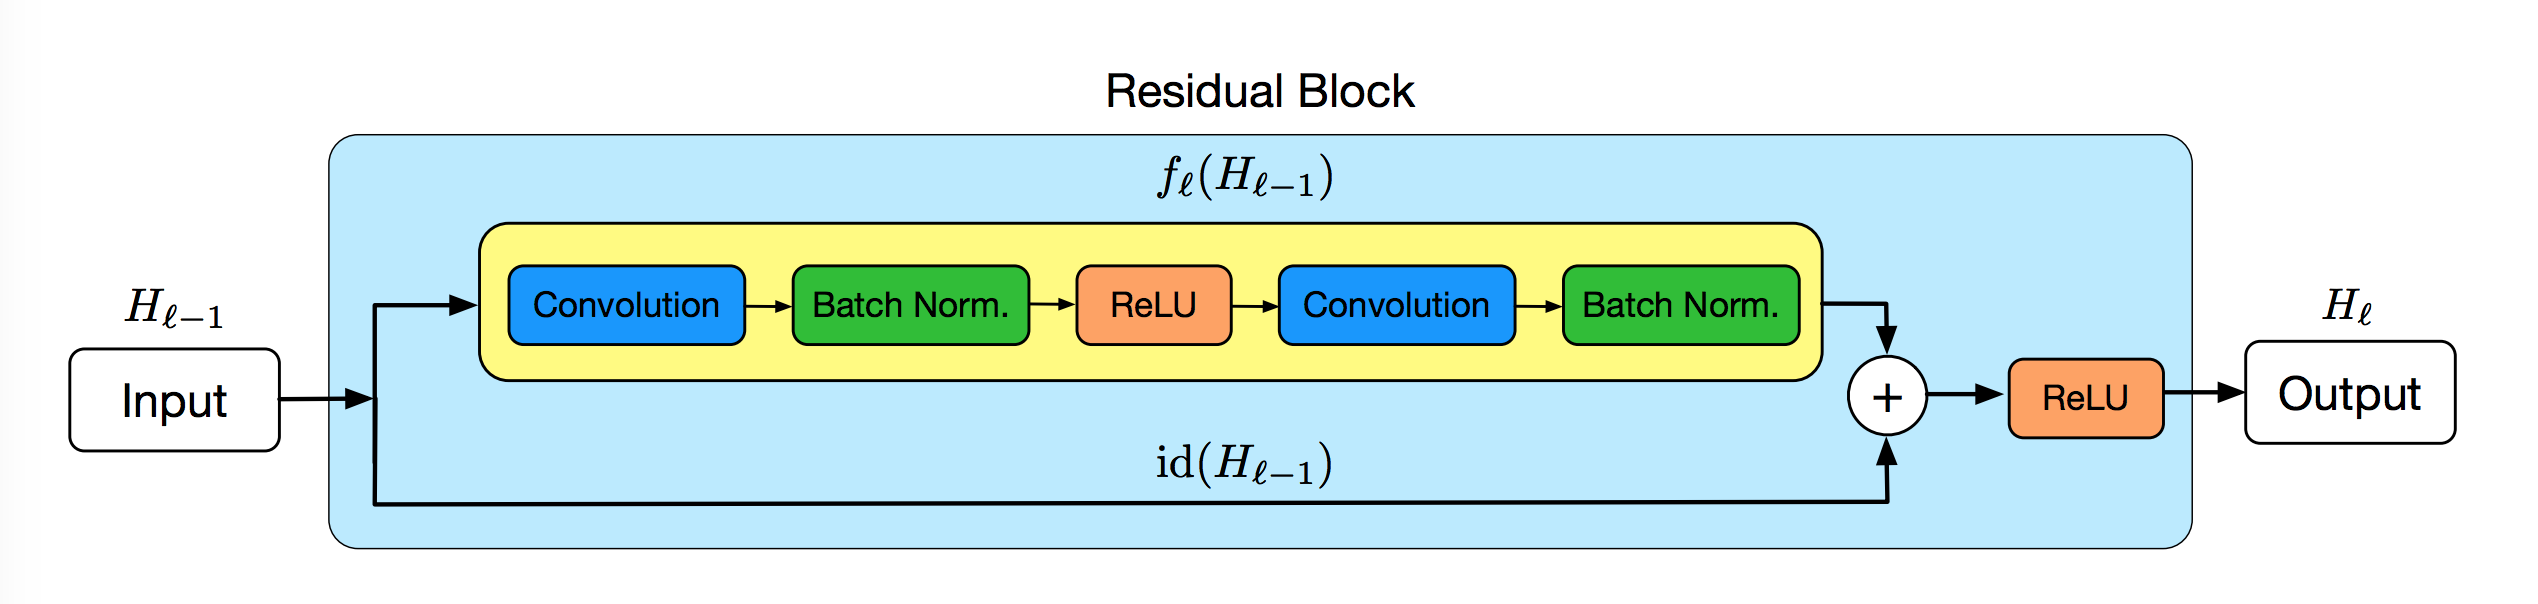
\includegraphics[width=0.9\paperwidth]{resnet_stoc.png}
%%\end{center}
%%
%%Обычный RESNET-блок: 
%%
%%\[
%%H_l = ReLU(f_l(H_{l-1}) + H_{l-1} ) 
%%\]
%%
%%\vfill %
%%\footnotesize 
%%\color{blue} \url{https://arxiv.org/abs/1603.09382}
%%\end{frame}
%%
%%
%%\begin{frame}{Нейросети со стохастической глубиной}
%%\begin{center}
%%	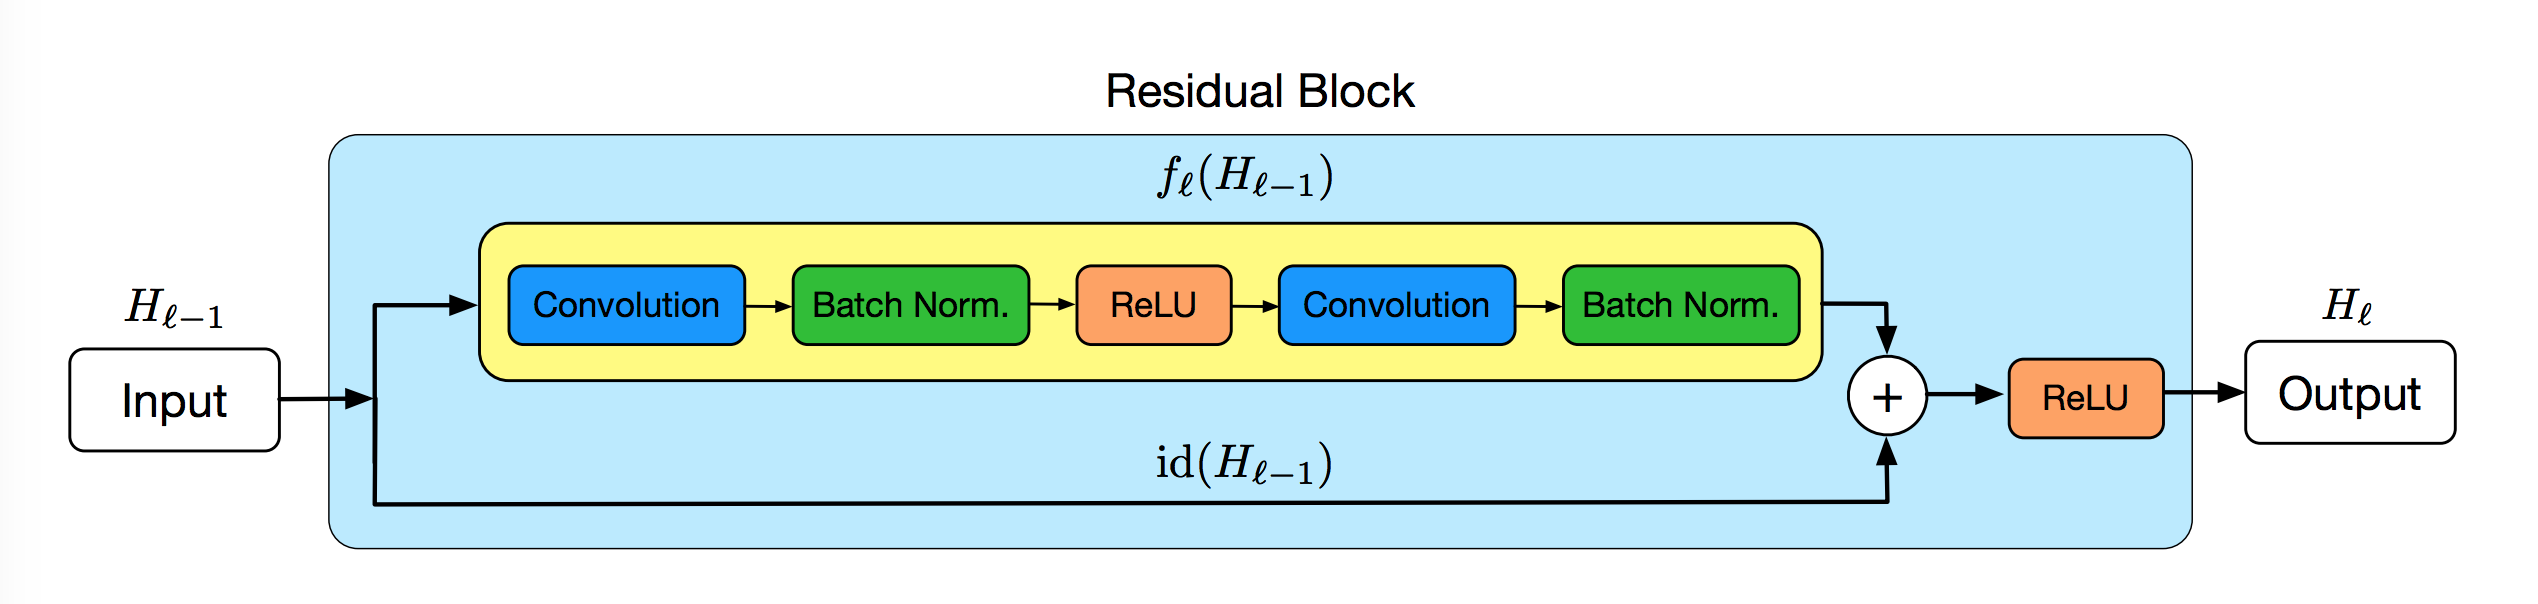
\includegraphics[width=0.9\paperwidth]{resnet_stoc.png}
%%\end{center}
%%
%%Немного видоизменим его: 
%%
%%\begin{equation*}
%%\begin{aligned}
%%& b_l \sim Bern(p_l) \\
%%& H_l = ReLU(b_l \cdot f_l(H_{l-1}) + H_{l-1} ) 
%%\end{aligned} 
%%\end{equation*}
%%
%%\vfill %
%%\footnotesize 
%%\color{blue} \url{https://arxiv.org/abs/1603.09382}
%%\end{frame}
%%
%%
%%\begin{frame}{Нейросети со стохастической глубиной}
%%\begin{wideitemize}
%%	\item  Для слоя $l$ мы задаём вероятность $p_l$, которая сохраняет этой слой в нейронной сетке
%%	
%%	\item Если $b_l = 1$, у нас остаётся обычный RESNET-блок, если $b_l = 0$ остаётся только skip-connection
%%	
%%	\item Глубина сетки зависит от того, как сгенирируется случайная величина
%%	
%%	\item Как подобрать $p_l$? 
%%	
%%	\item Первые слои важнее, так как они создают скрытые представления
%%\end{wideitemize}
%%\end{frame}
%%
%%
%%\begin{frame}{Нейросети со стохастической глубиной}
%%
%%\[
%%p_l = 1 - \frac{l}{L} \cdot (1 - p_L), \quad p_L = const \in [0;1]
%%\]
%%
%%\begin{center}
%%	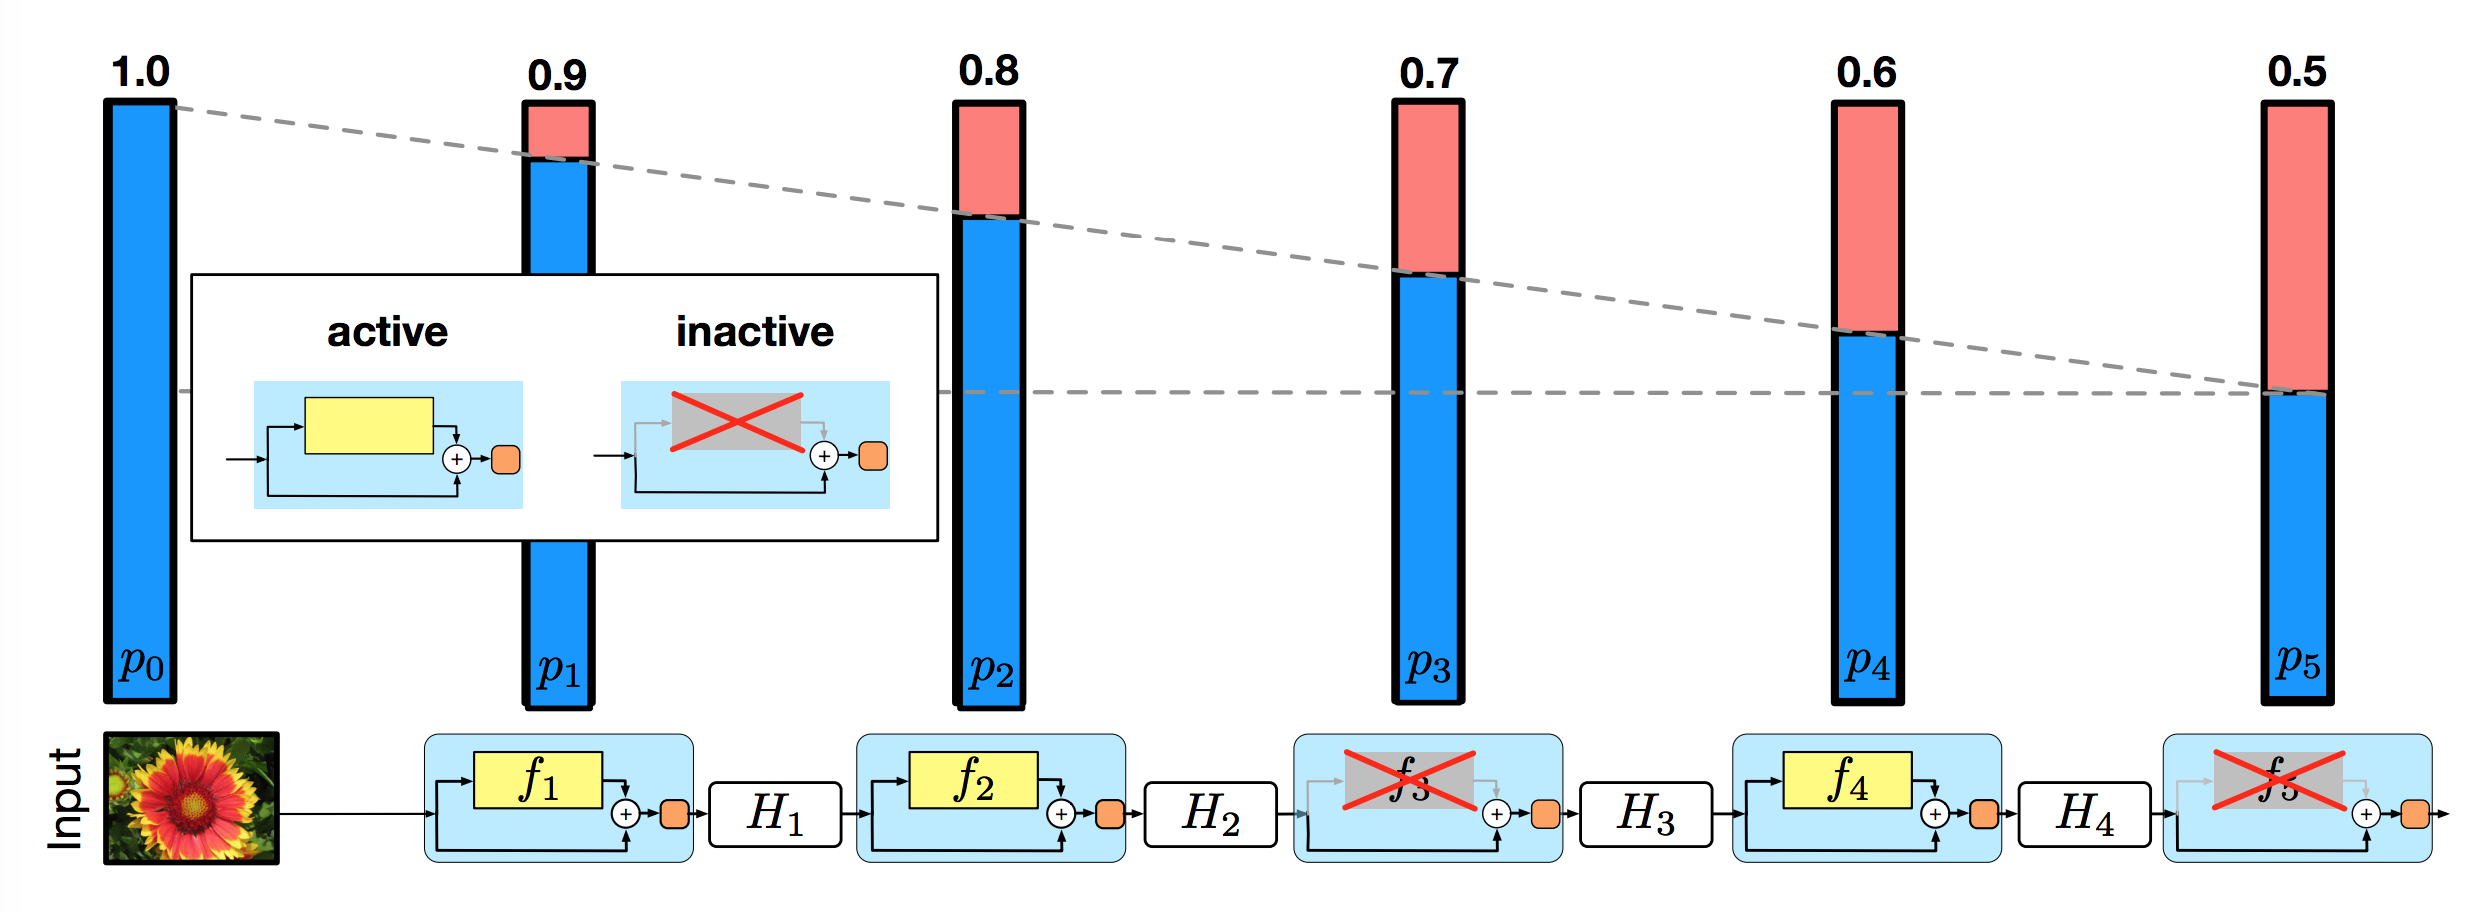
\includegraphics[width=0.9\paperwidth]{save_resnet.png}
%%\end{center}
%%
%%\vfill %
%%\footnotesize 
%%\color{blue} \url{https://arxiv.org/abs/1603.09382}
%%\end{frame}
%%
%%
%%\begin{frame}{Этап предсказания}
%%\begin{center}
%%	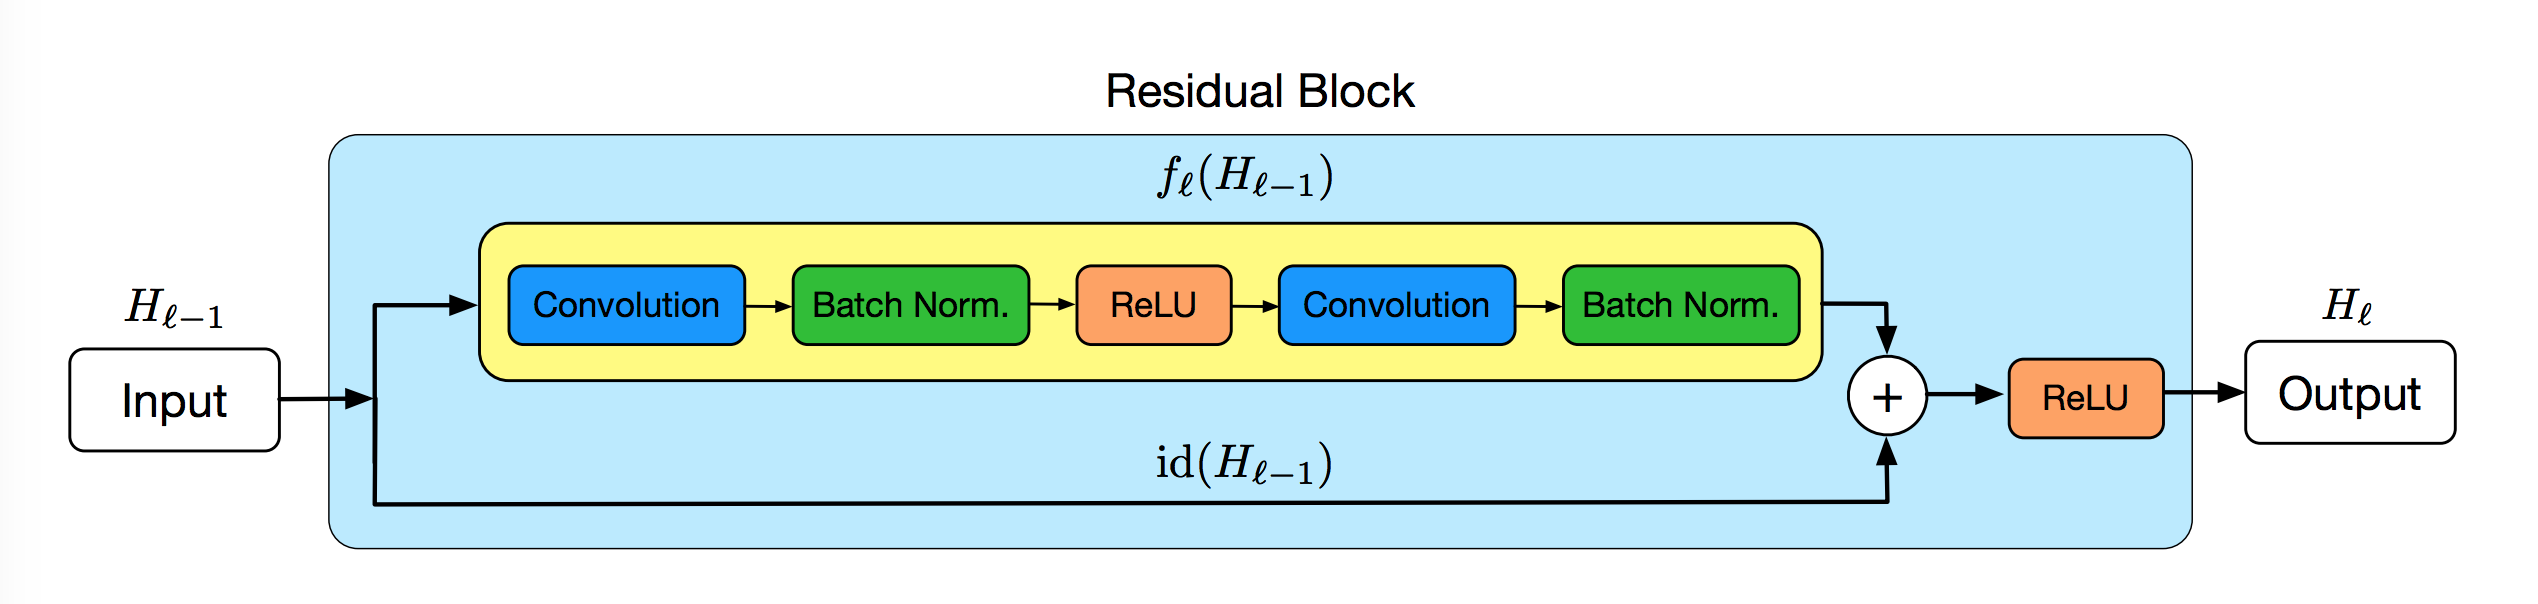
\includegraphics[width=0.9\paperwidth]{resnet_stoc.png}
%%\end{center}
%%
%%На этапе предсказания, пользуемся приёмом из Dropout. 
%%
%%\begin{equation*}
%%\begin{aligned}
%%& H_l^{test} = ReLU(p_l \cdot f_l(H^{test}_{l-1}) + H^{test}_{l-1} ) 
%%\end{aligned} 
%%\end{equation*}
%%
%%\vfill %
%%\footnotesize 
%%\color{blue} \url{https://arxiv.org/abs/1603.09382}
%%\end{frame}
%%
%%
%%\begin{frame}{Нейросети со стохастической глубиной}
%%\begin{center}
%%	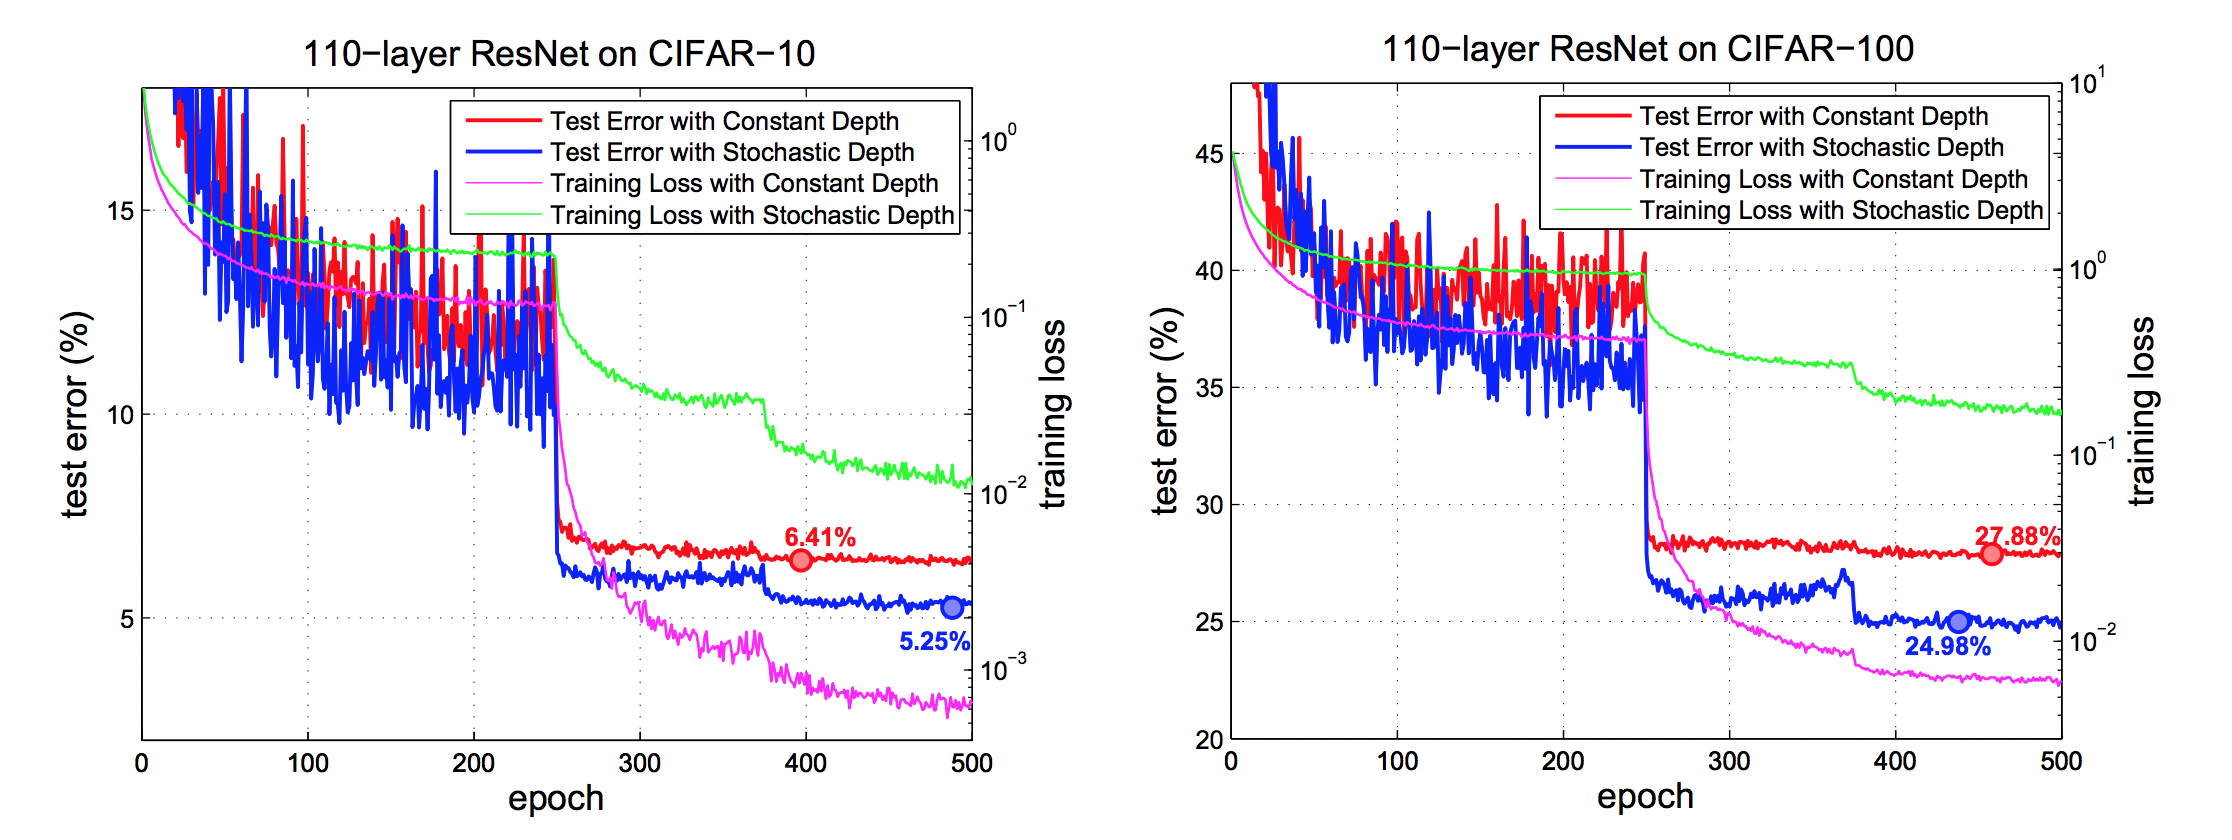
\includegraphics[width=0.9\paperwidth]{st_resnet_train.png}
%%\end{center}
%%
%%\vfill %
%%\footnotesize 
%%\color{blue} \url{https://arxiv.org/abs/1603.09382}
%%\end{frame}
%%
%%
%%\begin{frame}{Нейросети со стохастической глубиной}
%%\begin{wideitemize}
%%	\item  Сетка показывает более плохие показатели на тренировочной выборке, но выигрывает на тестовой
%%	
%%	\item Обучение из-за отсутствия некоторых блоков идёт быстрее
%%	
%%	\item Параметр $p_L$ отвечает за агрессивность выкидывания блоков, эксперименты показывают наилучшее качество сетки при $p_L = 0.5$
%%\end{wideitemize}
%%
%%\vfill %
%%\footnotesize 
%%\color{blue} \url{https://arxiv.org/abs/1603.09382}
%%\end{frame}


%%%\begin{transitionframe}
%%%	\centering 
\includegraphics[scale = 0.25]{eto-drugoe.png}
%%%	\begin{center}
%%%		\Huge  Какая-то хуета
%%%	\end{center}
%%%\end{transitionframe}

%%%\begin{frame}{Предобучение}
%%%\begin{wideitemize}
%%%	\item  Обучаем каждый нейрон на рандомной подвыборке, каждый нейрон впитает какие-то отдельные её особенности, после скрепляем все нейроны вместе и продолжаем обучение на всей выборке
%%%	
%%%	\item  \alert{На будущее:} обучаем на корпусе картинок автокодировщик, encoder благодаря этому учится выделять наиболее важные фичи, которые позволяют эффективно сжимать изображения. После срезаем decoder и на его месте достраиваем слои для решения нашей задаче, запускаем обычное дообучение.
%%%\end{wideitemize}
%%%\end{frame}
%%%
%%%
%%%\begin{frame}{Динамическое наращивание сети}
%%%\begin{wideitemize}
%%%\item  Обучение сети при заведомо недостаточном числе нейронов $H$
%%%\item После стабилизации функции потерь — добавление нового нейрона и его инициализация путём обучения 
%%%\begin{itemize}
%%%	\item либо по случайной подвыборке 
%%%	\item либо по объектам с наибольшими значениями потерь 
%%%	\item либо по случайному подмножеству входов
%%%	\item либо из различных случайных начальных приближений
%%%\end{itemize}
%%%\item Снова итерации BackProp
%%%\end{wideitemize}
%%%
%%%\vfill
%%%\begin{center}
%%%\alert{Эмпирический опыт:} Общее время обучения обычно лишь в $1.5-2$ раза больше, чем если бы в сети сразу было итоговое число нейронов. Полезная информация, накопленная сетью не теряется при добавлении нейронов.
%%%\end{center}
%%%\end{frame}
%%%
%%%
%%%\begin{frame}{Прореживание сети}
%%%\begin{wideitemize}
%%%\item Начать с большого количество нейронов и удалять незначимые по какому-нибудь критерию 
%%%\item \alert{Пример:} обнуляем вес, смотрим как сильно упала ошибка, сортируем все cвязи по этому критерию, удаляем $N$ наименее значимых
%%%\item После прореживания снова запускаем backprop
%%%\item Если качество модели сильно упала, надо вернуть последние удалённые связи 
%%%\end{wideitemize}
%%%\end{frame}

\end{document}